\documentclass[a4paper,11pt]{book}

\usepackage{impostazioni}

\begin{document}

\frontmatter
\begin{titlepage}
\newgeometry{top=2cm,bottom=2cm,left=2cm,right=2cm}
\vspace{5mm}
\begin{figure}[hbtp]
\centering

\includegraphics[scale=.43]{images/UNIPD.png}
\end{figure}
\vspace{5mm}
\begin{center}
{{\huge{\textsc{\bf UNIVERSIT\`A DEGLI STUDI DI PADOVA}}}\\}
\vspace{5mm}
{\Large{\bf Dipartimento di Fisica e Astronomia ``Galileo Galilei''}} \\
\vspace{5mm}
{\Large{\textsc{\bf Master Degree in Physics}}}\\
\vspace{20mm}
{\Large{\textsc{\bf Final Dissertation}}}\\
\vspace{30mm}
\begin{spacing}{3}
{\LARGE \textbf{Title}}\\
\end{spacing}
\vspace{8mm}
\end{center}

\vspace{20mm}
\begin{spacing}{2}
\begin{tabular}{ l  c  c c c  cc c c c c  l }
{\Large{\bf Thesis supervisor}} &&&&&&&&&&& {\Large{\bf Candidate}}\\
{\Large{\bf Prof./Dr. Name Surname}} &&&&&&&&&&& {\Large{\bf Name Surname}}\\
{\Large{\bf Thesis co-supervisor}}\\
{\Large{\bf Prof./Dr. Name Surname}}\\
\end{tabular}
\end{spacing}
\vspace{15 mm}

\begin{center}
{\Large{\bf Academic Year xxxx/xxxx}}
\end{center}
\end{titlepage}








\clearpage{\pagestyle{empty}\cleardoublepage}

\renewcommand{\baselinestretch}{1.2} 
\tableofcontents
\renewcommand{\baselinestretch}{1.5} 


\begin{abstract}
   
The ever evolving OT and IoT worlds continuously faces us with new challenges. One of this challenges is the ability in  
   
\end{abstract}

\mainmatter
%\chapter{Introduction}

The continuous evolution of the OT and IoT worlds constantly creates new challenges in the cyber security field. One of the main challenges directly derives from the evolution of the modern networks. With the advent of the Internet of Things many networks, especially in the industrial production field, that were once small and isolated from external devices are now becoming bigger and bigger and connected to the external world. This change brings with it many advantages such as the possibility of performing remote monitoring and surveillance but also many risks in terms of the security of the network itself.

One of the main challenges in the surveillance and control of a network is the capability of performing the so-called device identification, namely knowing which devices are connected to it. In small sized networks this operation can be executed "by hand" by singularly registering each connected device. In big scales networks where each day tens, if not hundreds, of devices are connected and disconnected, e.g. the Wi-Fi network of a company were the employees may connect with tables, laptops and smartphones, this operation must be automated. 

Connected devices provide some identifiers, such as the MAC address, in order to allow the manager of a network to identify them. This identifiers however are not always trustworthy, they can in fact be falsified and/or modified, mostly by users with malicious intentions. Alternative methods should then be implemented to identify what a connected device really is without using any modifiable information.

The goal of this work is to develop a method to identify a device using Machine Learning techniques and, in particular, Neural Network classifiers. In particular we want to develop an architecture able to identify, once trained, devices with high accuracy. We also want this architecture to be as flexible as possible, namely we want it to be able to perform its task over many different type of networks. 
%\chapter{Deep Learning and Neural Networks}

In the Machine Learning framework the so-called feature learning represents a class of methods whose goal is to create computing systems able to solve specific tasks, like detecting particular behaviours of structures or classifying a particular object, starting from the raw data.

Deep learning methods are a part of this family and have been applied in many fields, such as audio recognition and computer vision. Often this methods makes use of Artificial Neural Networks. Deep Learning is in fact usually referred to the use of Artificial Neural Networks with a multiple layer structure, from which the adjective 'deep' derives, as we will describe in the following.

\section{Artificial Neural Networks}

Artificial Neural Networks (ANNs in the following) are also denoted as biological-inspired networks; this denominations derives from their structure, which is inspired from  the brain of the animals. As for a natural brain, where each neuron communicates with others through the synapses, ANN are computing systems based on a series of units, called artificial neurons, connected among themselves. 

The simplest model used to represent an artificial neuron, capable of simple learning tasks, is the perceptron, invented in 1958 by Frank Rosenblatt\cite{perceptron}, whose work was inspired by the Warren McCulloch and Walter Pills\cite{nielsen}. A perceptron, given a series of binary input values $\bar{x}=\{x_1,\dots, x_n\}$, returns a single binary output value $f(\bar{x}, \alpha)$, where $\alpha$ are the internal parameters of the perceptron. 

The internal structure on the perceptron, represented in \figref{fig:perceptron}, is composed of a series of real-valued weights $\bar{w}=\{w_1,\dots,w_n\}$, a bias value $b$ and a threshold $\delta$. These parameters are used by the decision function $f$ to estimate the output value:

\begin{equation}
f(\bar{x},\alpha) = 
\begin{cases}
0\qquad\text{if}\quad\sum_{i=1}^N x_iw_i \leq \delta \\
1\qquad\text{if}\quad\sum_{i=1}^N x_iw_i > \delta \\
\end{cases}
\end{equation}

\begin{figure}[h]
    \centering
\includestandalone[height=6cm, width=\textwidth]{images/networks/perceptron}
\caption{Internal structure of a perceptron.}
    \label{fig:perceptron}
\end{figure}

\section{Neural Network architectures}

The perceptron model is unable to solve the complex tasks that are common nowadays in the Deep Learning field. In order to solve this tasks more complex models for the artificial neurons are used but, more importantly, the neurons are combined in order to create an Artificial Neural Network or ANN.

In most common applications the neurons are organized in consecutive layers.
In this structure each layer receives a series of values as input and produces an output which is used, with some manipulations, as input for the subsequent layer. The layers are usually denominated as following:
\begin{itemize}
    \item \textbf{Input Layer}: the first layer of the ANN, its input values are externally provided, i.e. an image for a classification task
    \item \textbf{Output Layer}: the last layer of the ANN, its output value is used as the prediction for the type of task the network is trying to solve
    \item \textbf{Hidden Layers}: all the intermediate layers of the network  
\end{itemize}

A first distinction in the structure of an ANN can be done between fully and partially connected ones. The former ones use as input of each neuron of a layer the output of all the neurons of the previous layer, the latter instead uses only a subset of those. A graphical representation of this difference is displayed in \figref{fig:full_part_ANN}.

\begin{figure}[h]
    \centering
    \begin{minipage}[c]{0.49\linewidth}
        \vspace{0pt}
        \centering
        \subfloat[Example of fully connected ANN structure]{
        \includestandalone[height=5cm, width=\textwidth]{images/networks/full_net}
            \label{fig:full_ANN}
        }
    \end{minipage}%
    \hfill%
    \begin{minipage}[c]{0.49\linewidth}
        \vspace{0pt}
        \centering
        \subfloat[Example of partially connected ANN structure]{
\includestandalone[height=5cm, width=\textwidth]{images/networks/partial_net}            \label{fig:part_ANN}
        }
    \end{minipage}%
    \caption{Graphical comparison of the architecture of a fully connected ANN and a partially connected one. The circles represent artificial neuron while grey lines indicate the connection between them.}
    \label{fig:full_part_ANN}
\end{figure}

An important aspect to highlight is that, due to the layered structure of the ANNs, we can disengage ourself from mathematically represent each single artificial neuron of the network and treat each  layer as a single mathematical object. \\
Given an ANN composed of $N_L$ consecutive layers, where the $i$-th layer is denoted with $L_i$, we can represent the output of a layer as a function:
\begin{equation}
    f_L^i (\bar{x_i})=a_i \left( \tilde{f}(\bar{x_i}, \boldsymbol{w}_i) + \bar{b}_i \right) 
    \label{eq:layer_math}
\end{equation}

where $\bar{x}_i$ is the input of the layer, $\boldsymbol{w}_i$ is a matrix of free parameters, called weights and $\bar{b}_i$ is a bias vector also composed of free parameters. The $\tilde{f}$ function is the key mathematical operation of the layer, whose choice leads to very different types of layers, which are then used to create specific types of ANNs, as described in \secref{ANN_type}. The $a_i$ function is the so-called activation function, whose choice plays a crucial role is the ability of the network to solve a specific task. Some of the possible choices for this function are reported in \secref{activations}.
This representation then allows us to represent an artificial neural network, composed of $N_L$ layers, as a set $\mathcal{F}_{N_L}$:
\begin{equation}
\mathcal{F}_{N_L} = \left\{ f_N(\bar{x}), \boldsymbol{w}, \bar{b}\right\}
\end{equation}

where $\boldsymbol{w} = \{\boldsymbol{w}_1 \dots \boldsymbol{w}_{N_L}\}$ and 
$ \bar{b} = \{ \bar{b}_1 \dots  \bar{b}_{N_L}\}$ are respectively the set of all the layer weight and biases and the $f_N(\bar{x})$ is the composition of the $f_L^i(\bar{x_i})$
functions:
\begin{equation}
    f_N(\bar{x}) = f_L^{N_L} \circ f_L^{N_L-1}\circ\dots\circ f_L^2\circ f_L^1 (\bar{x}) 
\end{equation}

Now that the structure of an ANN has been defined the most important question is how to find the best $\boldsymbol{w}$ and $\bar{b}$ parameters for a specific task.
Given a particular network structure and an input dataset $\mathcal{D}$, the best parameters  are estimated through a procedure called "training". In this procedure we define a loss function, which estimates how well the network is currently solving the task, and then utilize an algorithm which minimizes it by modifying the free parametes of the network. This steps are further explained respectively in \secref{lossfunction}
and \secref{weightoptimization}.

\subsection{Activation functions}\label{activations}

As shown in \forref{eq:layer_math} an ANN layer can be mathematically represented as:
\begin{equation}
    f_L^i (\bar{x_i})=a_i \left( \tilde{f}(\bar{x_i}, \boldsymbol{w}_i) + \bar{b}_i \right) 
    \label{eq:layer_math}
\end{equation}

where $a_i$ is the so-called activation function. The choice of this function plays a crucial role in determining both the capability of the network of solving the assigned task and also  the time needed for it to be able to solve it efficiently, namely different activation function may need a longer training than others. The choice of this function depends on various factors but the most important surely are the position of the layer inside the network and the specific task we are trying to solve.

The position inside the network is relevant since the hidden layers of the network are usually built using activation functions with output values in $\mathbb{R}$ or $\mathbb{R}^+$ while for the output layers activation functions with values in $[0,1]$ or $[-1,1]$ are preferred in order to interpret the results as a probability.
The specific task, on the other hand, mainly influences the activation function of the output layer since different tasks often requires a different output structure.
In the following a list of the most commonly used functions is presented.

\begin{figure}[!h]
\begin{minipage}{0.45\textwidth}
    \centering
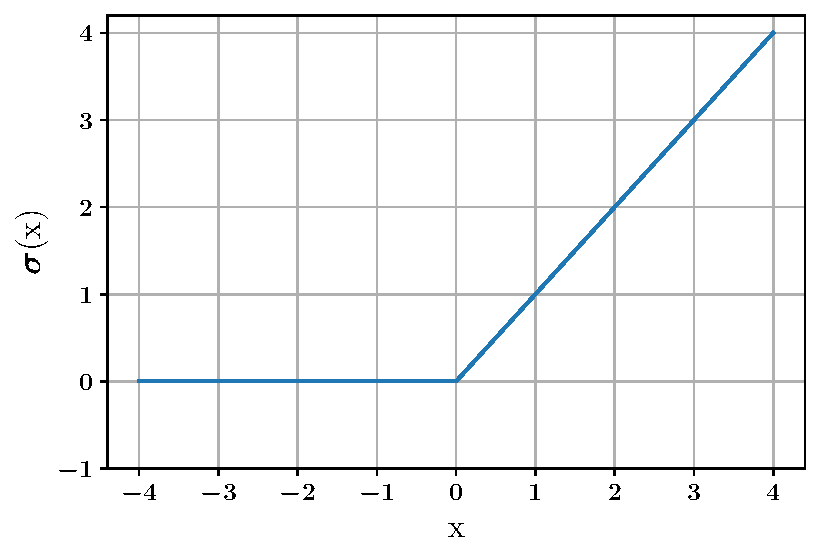
\includegraphics[width=\textwidth]{images/networks/act_relu.pdf}
\caption{ReLU activation function}
    \label{fig:act_relu}
\end{minipage}
\hfill
\begin{minipage}{0.5\textwidth}
    \textbf{Rectified Linear Unit (ReLU)}
   \begin{align}
        a(x) &=
        \begin{cases}
        x   & \text{if } x > 0 \\
        0  & \text{if } x \leq 0 
  \end{cases}
\end{align}
The ReLU is a continuous function with a point of non differentiability in 0. Despite being non differentiable this function is still implemented, mostly in the hidden layers of a network, due to its fast computation time. 
\end{minipage}
\end{figure}

\begin{figure}[!h]
\begin{minipage}{0.45\textwidth}
    \centering
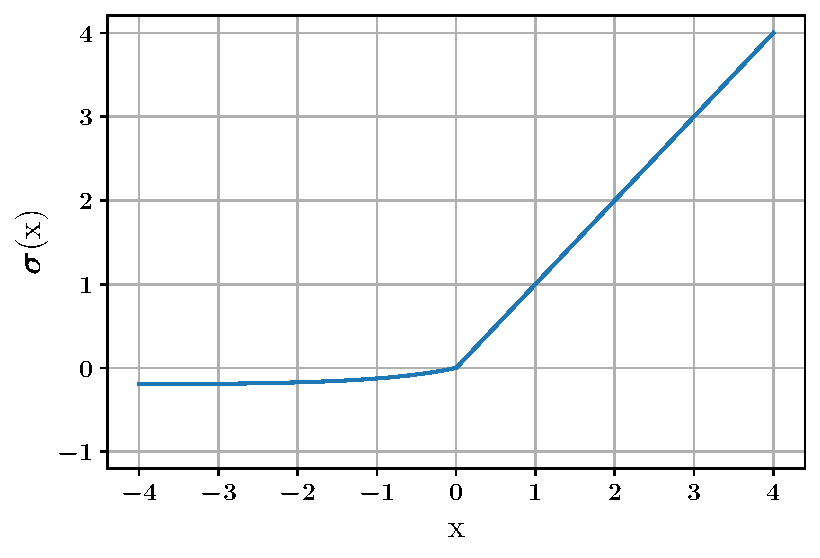
\includegraphics[width=\textwidth]{images/networks/act_elu.pdf}
\caption{ELU activation function}
    \label{fig:elu}
\end{minipage}
\hfill
\begin{minipage}{0.5\textwidth}
    \textbf{Exponential Linear Unit (ELU)}
   \begin{align}
        a(x) &= 
        \begin{cases}
        \alpha \left(e^x -1\right)  & \text{if } x \leq 0 \\
        x  & \text{if } x > 0 
  \end{cases}
\end{align}
The ELU activation functions is an improvement over the ReLU. In this case the negative values have an actual activation instead of being set to zero which may help the estimation of the network parameters. The drawback of choosing this function in an increase in the computational cost since an exponential operation is included. 
\end{minipage}
\end{figure}

\begin{figure}[!h]
\begin{minipage}{0.45\textwidth}
    \centering
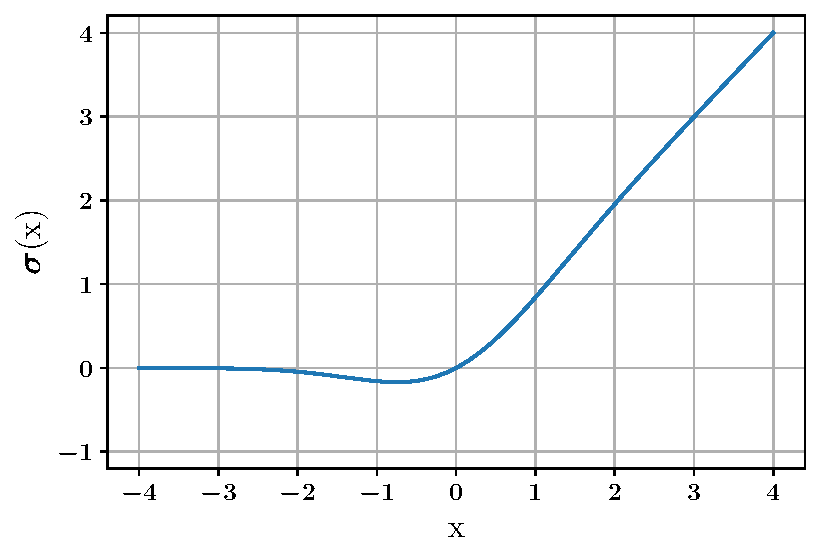
\includegraphics[width=\textwidth]{images/networks/act_gelu.pdf}
\caption{GELU activation function}
    \label{fig:gelu}
\end{minipage}
\hfill
\begin{minipage}{0.5\textwidth}
    \textbf{Gaussian Error Linear Unit (GELU)}
   \begin{equation}
       a(x) = \frac{1}{2} x \left( 1+\text{erf} \left( \frac{x}{\sqrt{2}}\right)\right)
   \end{equation}
   This is one of the newest activation functions. It was implemented in some of the most recent Deep Learining application proving to be one of the best activations in the Natural Language Processing field. 
\end{minipage}
\end{figure}

\begin{figure}[!h]
\begin{minipage}{0.45\textwidth}

    \centering
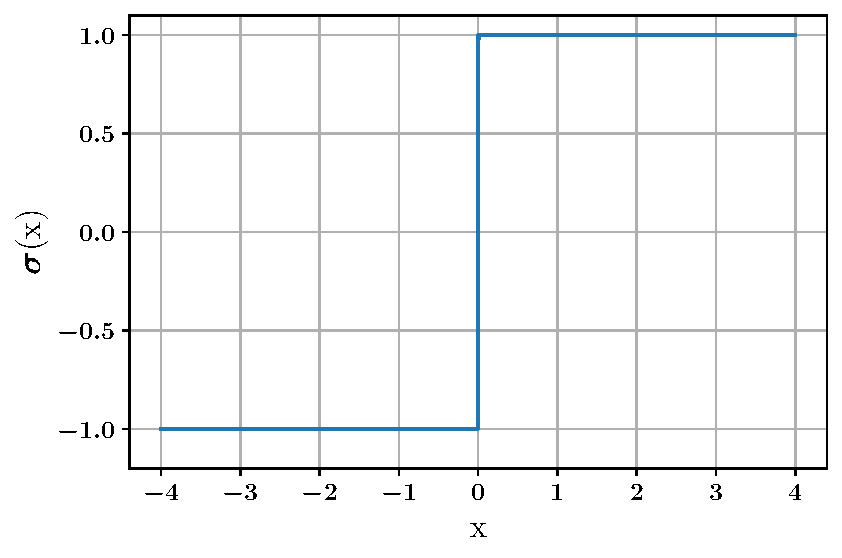
\includegraphics[width=\textwidth]{images/networks/act_step.pdf}
\caption{Step activation function}
    \label{fig:act_step}
\end{minipage}
\hfill
\begin{minipage}{0.5\textwidth}
    \textbf{Binary step}
      \begin{align}
        a(x) &=
        \begin{cases}
        1   & \text{if } x \geq 0 \\
        -1  & \text{if } x < 0 
  \end{cases}
\end{align}
Neurons using this function are also called linear threshold units(LTU). This type of neurons can be used for solving simple tasks but is not able to solve complex tasks like multiclass classifications or image recognitions.
\end{minipage}
    \end{figure}

\begin{figure}[!h]
\begin{minipage}{0.45\textwidth}

    \centering
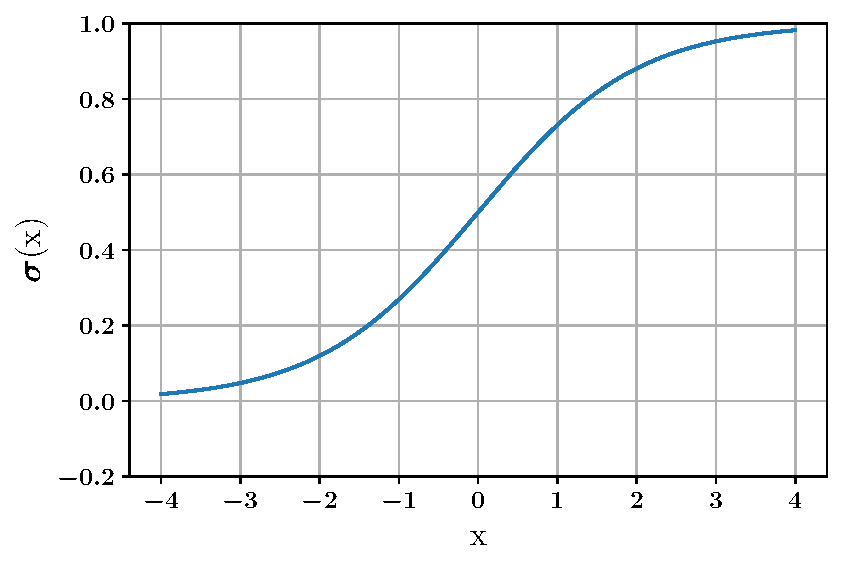
\includegraphics[width=\textwidth]{images/networks/act_sig.pdf}
\caption{Sigmoid activation function}
    \label{fig:act_sig}
\end{minipage}
\hfill
\begin{minipage}{0.5\textwidth}
    \textbf{Sigmoid} or \textbf{Soft step}
   \begin{equation}
       a(x) =\frac{1}{1+e^{-x}}
   \end{equation}
   The sigmoid functions provides an output value in $[0,1]$ and is differentiable in every point. This properties makes it one of the most used activation functions for the last layer of an ANN.
\end{minipage}
    \end{figure}


\begin{figure}[!h]
\begin{minipage}{0.45\textwidth}
    \centering
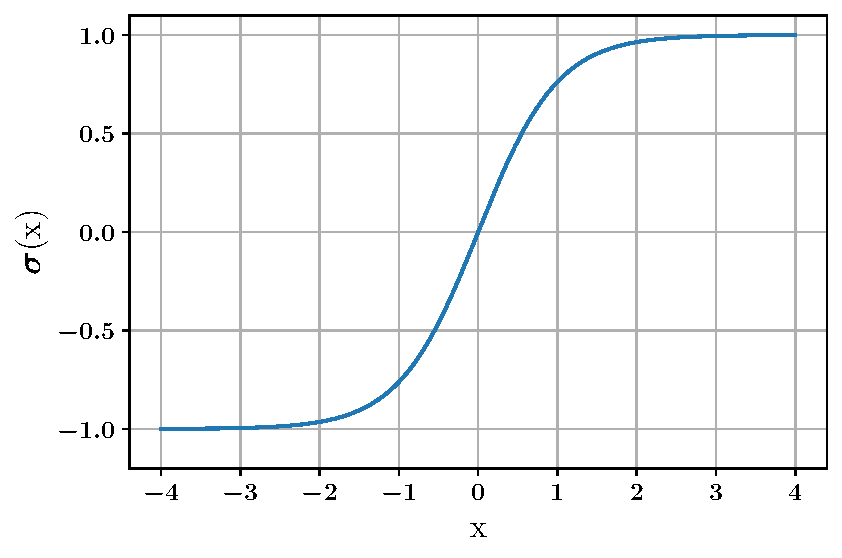
\includegraphics[width=\textwidth]{images/networks/act_tanh.pdf}
\caption{Hyperbolic tangent activation function}
    \label{fig:act_tanh}
\end{minipage}
\hfill
\begin{minipage}{0.5\textwidth}
    \textbf{Hyperbolic tangent}
   \begin{equation}
       a(x) =\frac{e^x-e^{-x}}{e^x+e^{-x}}
   \end{equation}
The hyperbolic tangent has similar properties to the sigmoid function. Its output is however in $[-1,1]$ which may speed up convergence in same applications.
\end{minipage}
\end{figure}

 

\section{Types of Artificial Neural Network and layer structure}
\label{ANN_type}

As described in the previous section, a layer of an ANN can be represented by its key mathematical operation. In the most common applications this operation is a function depending of the input vector of the layer and of a series of free parameters called weights.

The choice of this operation is of fundamental importance since the whole behaviour of an ANN depends on it. More specifically the choice of this operation determines the type of the layer and, consequently, the type of ANN we are creating. 

There are many possible choices and architectures but, for this work, we will focus on the main two type of Artificial Neural Networks and their type of layers: Dense Neural Networks and Convolutional Neural Networks, respectively described in \secref{dnn} and \secref{cnn}.
It is important to highlight that, despite being described separately, this two architectures can be combined together, as we will see in the following chapters, in order to create a better predictor.

\subsection{Dense Neural Networks}\label{dnn}

Dense neural networks, also known as DNNs, are Artificial Neural Networks with many fully connected hidden layers between the input and output ones, this result in a high number of connections between the units from which the 'dense' adjective derives.

Following directly from this denominations the fully connected layers that compose a Dense Neural Network are called Dense Layers.
A dense layer, whose decision function will denoted with $f_D$, is characterized by the dot product $\cdot$ as its key mathematical operation, using the notation previously introduced it can then be represented as:
\begin{equation}
    f_D (\bar{x})=a_i \left( \bar{x} \cdot \boldsymbol{w} + \bar{b}_i \right) 
    \label{eq:layer_dense}
\end{equation}

Depending on the structure of the input vector $\bar{x}$ and on the weight tensor $\boldsymbol{w}$ the dot product represent a different mathematical operation, specifically:
\begin{itemize}
    \item if both $\bar{x}$ and $\boldsymbol{w}$ are 1-dimensional vectors the dot product corresponds to the inner product of the two
    \item if both $\bar{x}$ and $\boldsymbol{w}$ are 2-dimensional, namely they are matrices, the dot product corresponds to the matrix-matrix multiplication of the two
     \item if either one is a scalar value then the dot product corresponds to a simple multiplication where the scalar is used as a factor
     \item if $\bar{x}$ and $\boldsymbol{w}$ respectively are an N-dimension and M-dimension tensor the dot product becomes a sum product over their last dimensions
\end{itemize}

In \figref{fig:dnn_example} an illustration of the structure of a simple DNN is reported. DNNs are commonly used to solve many tasks but the field in which they are mostly implemented is the classification, due to their ability of easily understanding both linear and non-linear patterns in a multi-variate analysis.


\begin{figure}
    \centering
\includestandalone[width=0.8\textwidth]{images/networks/DNN}
    \caption{Example of the structure of a Dense Neural Network. The neurons of each layer are represented by circles while the grey lines represent connections between them.}
    \label{fig:dnn_example}
\end{figure}

One of the main drawbacks of the usage of DNNs is however the number of free parameters. Dense layers are in fact characterized by an high number of weights and, due to the fully connected structure of the network, the total number of parameters grows really fast with each additional layer. 
A too high number of parameters may lead to two main issues. The first problem one may encounter is the inability of the network to correctly estimate the optimal parameters, resulting in its inability of giving correct prediction. The second possible issue is the so-called over-fitting problem, namely the network adapts too well to the data on which its train is performed, but again gives completely wrong prediction when tested on other data. A brief explanation of this issue is discussed in \secref{fit_over_under}.
To avoid this issues the number of free parameters can be controlled, working on two factors: the shape of the input vector, which depends on the specific tasks but can sometimes be modified or reduced using techniques such as the PCA, and the number of neurons in each layer, which can be selected in order to reach the best compromise between performances and model complexity.

\subsection{Convolutional Neural Networks}\label{cnn}

Another type on ANN is the so-called Convolutional Neural Network, also known as CNN. As the name suggests the key mathematical operation in the layers of this type of network is the convolution, this layers are therefore called Convolutional Layers, from which the CNN name derives.

The key elements of a convolutional layers are the so-called filters. The output of a convolutional layer is fact computed as the resulting vector of the discrete convolution of the input values with each filter. 

\begin{wrapfigure}{r}{0.5\textwidth}
    \centering
  \includestandalone[width=0.5\textwidth]{images/networks/CNN}
    \caption{Example of the combination of a convolutional layer with one 1 dimensional filter and a max pooling layer performing.  }
    \label{fig:cnn_tot}
    \vspace{-1cm}
\end{wrapfigure}
The filters of a CNN have the same role of the weight tensor of a DNN and are in fact the free parameters of the network, whose optimization is performed during the training. In \figref{fig:cnn_filter} an example of the result of the application of a filter to a 2-dimensional input is shown.

In most of the common implementations however CNNs are not composed of only convolutional layers but are made of an alternation of convolutional and pooling layers, where the latter is used to  perform a non-linear down-sampling on the output of a convolutional layer. An example of the combination of these two layers is shown in \figref{fig:cnn_tot}.
More specifically a pooling layer divides its input in a series of region called "pools" and applies a function to each one.
The resulting value from all pools is then combined and used as the output of the layer.


Many choices for both the size of the pools and the function to apply are possible however one of the most common implementation is a max-pooling layer with a 2x2 pool size, namely a layer that divides the input in 2x2 regions and takes the highest value from each of them. A example of the application of this type of layer is shown in \figref{fig:cnn_pool} 

\begin{figure}[h]
    \centering
      \includestandalone[ width=\textwidth]{images/networks/cnn_filter}
    \caption{Example of the application of a filter over a 2 dimensional input. The resulting matrix is computed as the discrete convolution of the input with the filter values.}
    \label{fig:cnn_filter}
\end{figure}

\begin{figure}[h]
    \centering
     \includestandalone[ width=0.78\textwidth]{images/networks/cnn_pool}
    \caption{Example of the application of the max pooling operation over a 2 dimensional input, with 2x2 pool size. The resulting matrix is computed as the maximum value of each 2x2 pool.}
    \label{fig:cnn_pool}
\end{figure}


%\begin{wrapfigure}{r}{0.5\textwidth}
%    \centering
%  \includestandalone[height=7cm, width=0.6\textwidth]{images/networks/CNN}
%    \caption{cnn }
%    \label{fig:cnn_tot}
%\end{wrapfigure}


\section{Loss functions} \label{lossfunction}

After the choice of the ANN type and its internal structure the next step is to choose the so-called loss function, also known as risk or cost function\cite{lossfunc}. The role of the loss function is to quantify how well the predicting power of the network is and its choice plays a crucial role in the learning procedure.

In most Deep Learning application the role of the learning algorithm is in fact to estimate the best set of parameters that are able to minimize the value of the loss function over a set of given input values. The choice of this function is therefore really important since it may greatly influence the final ability of the model of producing correct predictions.

As for the activation functions many choices of the loss function are possible. In the following part we present a brief list of the ones implemented in the most common applications:
\begin{itemize}
    \item \textbf{Mean Squared Error} or \textbf{L2 Loss}:\\
    This loss computes the average of the squared distance between the correct label associated to a sample, $y_{i,T}$ and the predicted one, $y_{i,P}$:
    \begin{equation}
        L_{MSE}= \frac{1}{N}\sum_{i=1}^N \left(y_{i,T}-y_{i,P}\right)^2
    \end{equation}
    This function is mostly implemented in regression tasks and is characterized by the heavy penalization imposed on predicted values very distant from their correct label. 
    \item \textbf{Mean Absolute Error} or \textbf{L1 Loss}:\\
    This loss computes the average of the absolute distance between the correct label associated to a sample, $y_{i,T}$ and the predicted one, $y_{i,P}$:
    \begin{equation}
        L_{MAE}= \frac{1}{N}\sum_{i=1}^N \left|y_{i,T}-y_{i,P}\right|
    \end{equation}
    Similarly to the L2 loss also the L1 is used in regression tasks but it penalizes more many small deviation from the correct label than few very distant ones. The main drawback of the L1 loss is the necessity of more complex tools for the computations of the gradient, with respect to the L2 loss, whose gradient can be easily computed exploiting its mathematical properties. 
\item \textbf{Hinge Loss}:\\
    The hinge loss is mostly famous for its implementation in Support Vector Machines (SVMs). As for the previous losses the Hinge one is a function of the true, $y_{i,T}$ and  predicted label, $y_{i,P}$ but with the constraint of them being either $\pm 1$:
    \begin{equation}
        L_{H}= \sum_{i=1}^N \max\left( 1-y_{i,T}*y_{i,P},0\right)
    \end{equation}
\item \textbf{Binary Cross Entropy Loss}:\\
    This function is the standard loss implemented for the binary classification tasks. It is computed using the true label associated to the i-th sample, requested to be a binary value, $y_{i,T}\in{0,1}$ and the probability $p_{i}$ of it being associated to the class indicated with $y_{T}=1$. With this notation the loss function is written as:
    \begin{equation}
        L_{BCE}= -\sum_{i=1}^N\left[ y_{i,T}\log(p_i)+
        \left(1- y_{i,T}\right)\log(1-p_i)\right]
    \end{equation}
    This loss function heavily penalizes confident but wrong predictions. 
\item \textbf{Categorical Cross Entropy Loss}:\\
    This loss function is the natural generalization of the previous one. As such it is the standard function implemented in multi-class classification tasks. Considering a classification tasks with $M>2$ classes, we can define: 
    \begin{equation}
        L_{CCE} = -\sum_{i=1}^N \sum_{c=1}^M  \left[
        y_{i,c}\log(p_{i,c}) + (1-y_{i,c})\log(1-p_{i,c})
        \right]
    \end{equation}
    where $p_{i,c}$, represent the predicted probability of the i-th belongin to the class $c$ and $y_{i,c}$ is a binary number equal to 1 only for the true class of the sample.
\item \textbf{Kullback-Leibler Divergence}:\\
   This loss function, commonly used in mathematical statistic as a difference measure between distribution, has proven its efficiency also for Deep Learning methods\cite{kullbackeff, kullbackeff2}. Indicating with $p_i$ and $q_i$ respectively the predicted and true label of a sample:
    \begin{equation}
        L_{KL} = - \left( \sum_{i=1}^{M} p_{i} \log{q_{i}} - \sum_{i=1}^{M} p_{i} \log{p_{i}} \right)
    \end{equation}
    
\end{itemize}


\subsection{Overfitting and underfitting recognition} \label{fit_over_under}

Aside from being the quantity used to estimate the optimal parameters of a predictor the loss function is also used to monitor the performance in search of over and under fitting behaviour during the learning procedure. 
This issues can be observed dividing the given dataset $\mathcal{D}$ in two parts: a training dataset $\mathcal{D}_{TR}$ and a test dataset $\mathcal{D}_{TE}$\footnote{In many applications the dataset is not split in two but rather three subsets, namely the training $\mathcal{D_{Tr}}$, validation $\mathcal{D_{V}}$ and test $\mathcal{D_{Te}}$ set. In this case the validation set is used to monitor the eventual presence of over and under fitting while the test set is used to evaluate the final performance of the model. As we will see in the following chapters this strategy of division is also the one implemented in this work.}. As the name suggests the training dataset is used to train the predictor while the test set is used to verify the effective performance after the learning.

The overfitting\cite{overfitting} issue is observable in cases where the prediction model adapts too well to the training set, failing to give good predictions on the test set. This issue is common in cases where the complexity of the model is too high compared to the size or structure of the given dataset or when the training is performed for too long. Possible ways to resolve the overfitting issue are using a simplified model or using some optimization techniques, such as the regularization and dropout, described in \secref{opt_tec}.
The opposite of the overfitting is the so-called under fitting. This issue arises whenever there is still room for improving the model prediction capability. Possible ways to resolve this issue is the introduction of a more complex model or just increasing the training time.

In order to visualize this two issues, lets for example consider the simple task of performing a polynomial fit over a given distribution, as shown in  \figref{fig:overunderfit}. The data samples in this figure have been generated from a second degree polynomial distribution plus some gaussian noise and divided in training, over which the fit is performed, and test samples. The distribution is then fitted with a first, second and 10-th degree polynomial and the MSE Loss, introduced before, is computed. As we can see the second order polynomial fit has similar training and the fit well represents both the distribution. On the other hand the first order fit instead has a very high training and test error which is a clear sign of the underfitting issue. Finally the 10-th order polynomial fit presents a very low training error and an high test error which indicates that the estimated distriubution is overfitted on the training set but does not represent effectively the full distribution.

\begin{figure}[h]
    \centering
    \begin{minipage}[c]{0.49\linewidth}
        \vspace{0pt}
        \centering
        \subfloat[1st order polynomial fit]{
        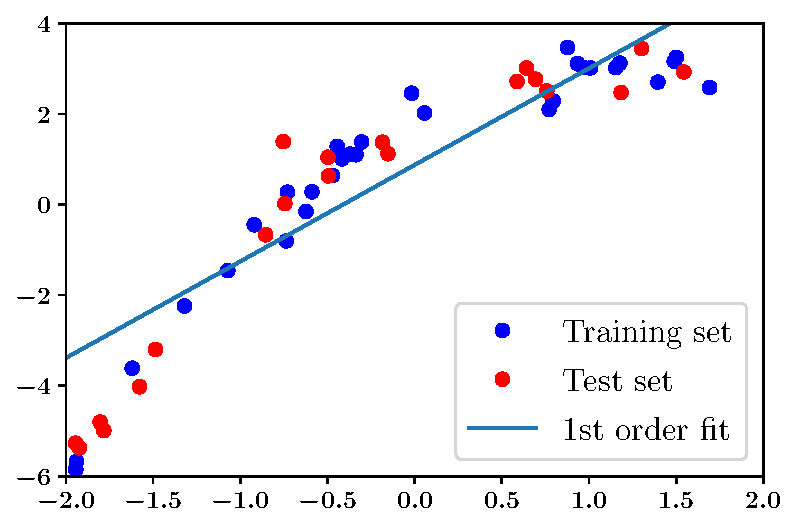
\includegraphics[width=\textwidth]{images/networks/over_under_fit_p1.pdf}
            \label{fig:p1_fit}
        }
    \end{minipage}%
    \hfill%
    \begin{minipage}[c]{0.49\linewidth}
        \vspace{0pt}
        \centering
        \subfloat[2nd order polynomial fit]{
        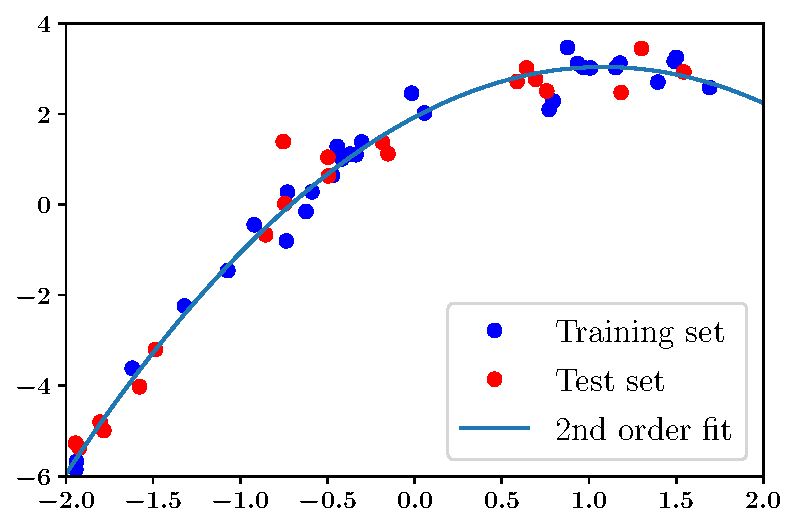
\includegraphics[width=\textwidth]{images/networks/over_under_fit_p2.pdf}
            \label{fig:p2_fit}
        }
    \end{minipage}%
    
    \begin{minipage}[c]{0.49\linewidth}
        \vspace{0pt}
        \centering
        \subfloat[10th order polynomial fit]{
        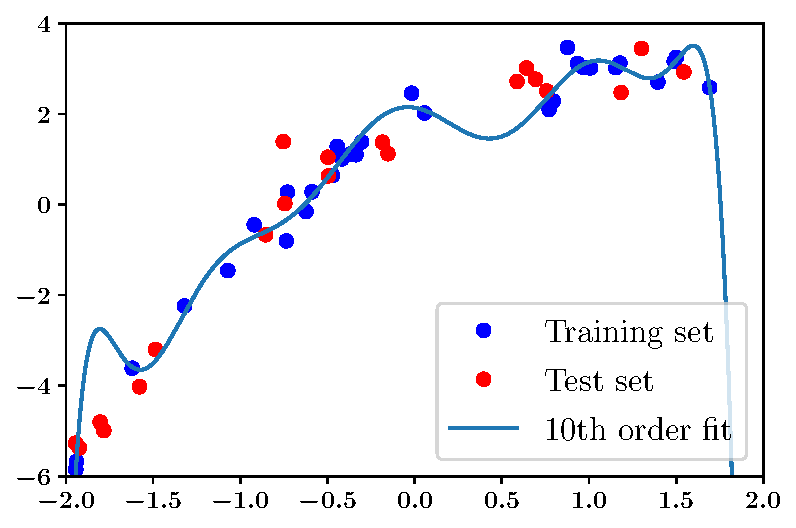
\includegraphics[width=\textwidth]{images/networks/over_under_fit_p10.pdf}
            \label{fig:p10_fit}
        }
    \end{minipage}%
    \hfill%
    \begin{minipage}[c]{0.49\linewidth}
        \vspace{0pt}
        \centering
        \subfloat{
            \begin{tabular}{ccc}
            \toprule
                 & \multicolumn{2}{c}{\textbf{Mean Squared Error}}  \\
            \textbf{Fit order} & \textbf{Train} & \textbf{Test} \\
            \midrule
            1$^\text{st}$ &  1.11 & 1.57 \\
            2$^\text{nd}$ &  0.11 & 0.17 \\
            10$^\text{th}$ &  0.06 & 0.93 \\
            \bottomrule
            \end{tabular}
            \label{tab:fitmse}
        }
    \end{minipage}%
    \caption{Over and underfitting issue in polynomial regression over a set of randomly generated samples. Samples are divided in training set, used for the regression and test set, used to compute the goodness of the fit.
    The fit is performed using a 1$^\text{st}$, 2$^\text{nd}$ and 10$^\text{th}$ degree polynomial, respectively shown in \figref{fig:p1_fit}, \figref{fig:p2_fit} and \figref{fig:p10_fit}. The mean squared error computed over both the training and test set is also reported. }
            \label{fig:overunderfit}
\end{figure}







%\begin{figure}
%    \centering
%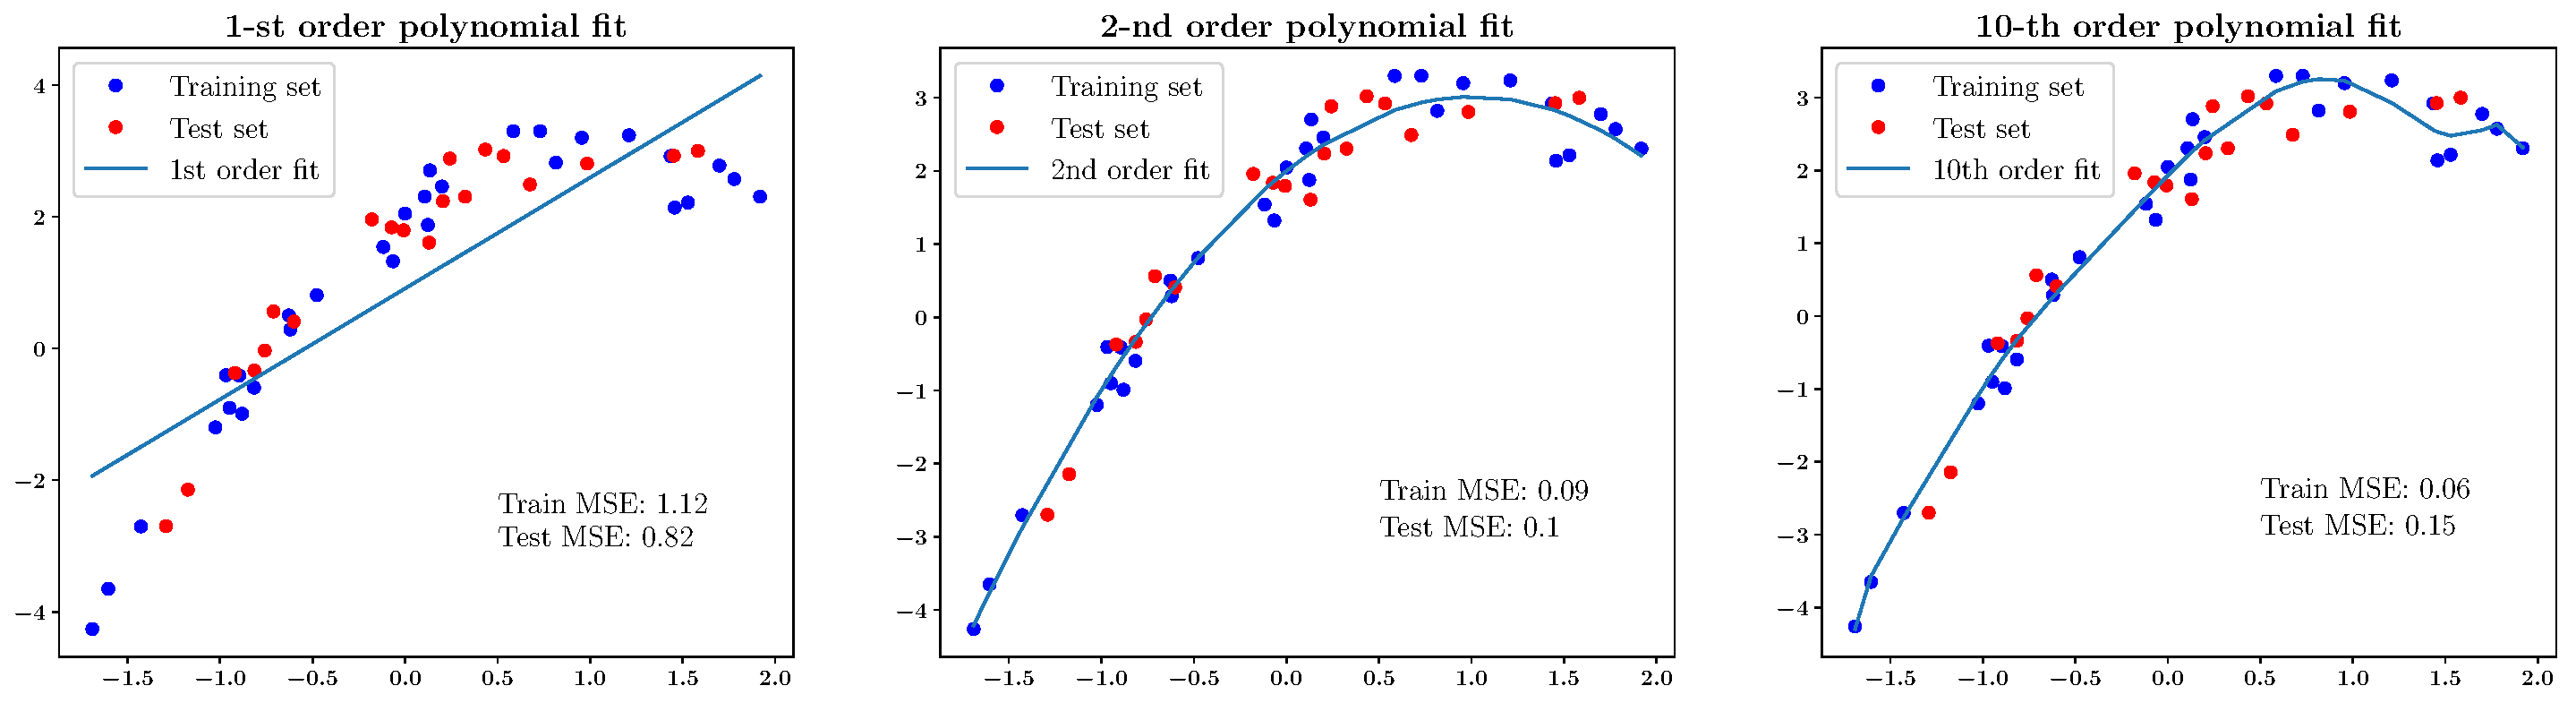
\includegraphics[width=\textwidth]{images/networks/over_under_fit.pdf}
%\caption{overunder fit }
%    \label{fig:overunderfit}
%\end{figure}

\section{Network parameters optimization}\label{weightoptimization}

We have now illustrated the main choices for the creation of an ANN and for the loss function. We know focus on how ann ANN can be trained in order to give relevant prediction respect to the task we are able to solve. 
As we saw in the previous section an ANN is composed by a set of free parameters, namely the weights and biases. The goal of our algorithm is then to find the best parameters able to minimize the value of the selected loss function. This is done using the so-called Backpropagation algorithm\cite{backprop}, described in \secref{backprop}. This algorithm provides a solid method to compute the gradient of the loss function with respect to the free parameter. The gradient of the loss function is then utilized to update the values of the weights and biases themselves through an optimization algorithm, such as the ones described in \secref{optalg}.
These algorithms are iterated over the full network until a condition, which usually is a maximum number of iterations or a minimum loss value, is met. Each complete iteration of the full gradient estimation and parameter updating is called epoch.

\subsection{Backpropagation algorithm}\label{backprop}

The backpropagation algorithm is divided in two procedures: the Forward propagation and the Back computation.
The Forward propagation corresponds to the computation of the loss function $L(\bar{y}_p, \bar{y}_t)$, where $\bar{y}_p$ is the set of predicted labels, produced by the ANN over an input dataset $\mathcal{D}$, and $\bar{y}_t$ is the set of true labels. 
After the forward propagation is done the backward computation is performed. In this procedure the information from the loss function is propagated backward and used to numerically compute the gradient of the loss function with respect to the free parameters. This allows to easily compute a quantity that would instead take long and difficult analytical computation to be estimated.
More specifically the procedure first computes the gradient of the loss function with respect to each layer and, starting from this values, it estimates the gradient with respect to the single parameter.
The pseudoce of the two procedures is respectively reported  in \algoref{alg:fow_prop} and \algoref{alg:back_comp}, for the forward propagation and backward substitution. 

\begin{algorithm}
\caption{Pseudo-code illustration of the forward propagation procedure for the computation of the predicted labels $\bar{y}_p$ and of the loss function $L(\bar{y}_p,\bar{y}_t)$. In the algorithm the symbol $a^{(i)}$ indicates the activation function of the i-th layer, $f^{(i)}$ its key mathematical operation of the layer and $z^{(i)}$ its output.}
\label{alg:fow_prop}
\begin{algorithmic}[1]
\Require $N_L$ \Comment Depth of the network
\Require $\mathbf{w}^{(i)}$, $i \in \{1,\dots,N_L\}$ \Comment Weight parameters of the network
\Require $b^{(i)}$, $i \in \{1,\dots,N_L\}$ \Comment Bias parameters of the network
\Require $\bar{x}$ \Comment Input value for the prediction
\Require $\bar{y}_t$ \Comment true labels associated to $\bar{x}$

\Procedure{Forward Propagation}{$x$}%\Comment{The g.c.d. of a and b}

\State $z^{(0)} = x$

\For{$k=1,\dots,N_L$} \Comment Loop over the layers
\State $t^{(k)} = b^{(k)} + f^{(k)}\left(\mathbf{w}^{(k)}, z^{(k-1)}\right)$ \Comment Compute operation and apply bias
\State $z^{(k)} = a^{(k)}(t^{(k)})$ \Comment Apply activation function
\EndFor

\State $\bar{y}_p = z^{(N_L)}$

\State \textbf{return} $\hat{y}$, $L(\bar{y}_p,\bar{y}_t)$ \Comment Return predicted labels and loss computation 
\EndProcedure
\end{algorithmic}
\end{algorithm}


\begin{algorithm}
\caption{Pseudo-code illustration of the backward propagation procedure for the computation of the loss gradient respect to each layer. In the algorithm we indicate with $\bar{y}_p$ and $\bar{y}_t$ respectively the set of predicted and true labels. From the \algoref{alg:fow_prop} we use the notation $z^{(k)}$ to indicate the output of a layer and all the values computed in \algoref{alg:fow_prop} are intended as available to the procedure.}
\label{alg:back_comp}
\begin{algorithmic}[1]

\Procedure{Backward Computation}{$x$} \Comment After the forward computation

\State $g \gets \nabla_{\hat{y}}L = \nabla_{\bar{y}_p}L(\bar{y}_p,\bar{y}_t)$\Comment Compute the gradient on the output layer

\For{$k=N_L,N_L-1,\dots,1$}
\State $g \gets \nabla_{t^{(k)}}L = g \odot a^{(k)\prime}(t^{(k)})$
\State $\nabla_{b^{(k)}}L = g$ \Comment Gradient w.r.t biases
\State $\nabla_{\mathbf{w}^{(k)}}L = g z^{(k-1)~T}$ \Comment Gradient w.r.t weight
\State $g \gets \nabla_{z^{(k-1)}}L = \mathbf{w}^{(k)~T} g$ \Comment Gradient w.r.t previous layer
\EndFor

\State \textbf{return} $\nabla_{b^{(k)}}L$, $\nabla_{\mathbf{w}^{(k)}}L$ $\quad$ for $k \in \{1,\dots,N_L\}$ \Comment Return the gradients
\EndProcedure
\end{algorithmic}
\end{algorithm}



\subsection{Optimizers}\label{optalg}

Once the gradient, with respect to each parameter, is computed we can update the parameters themselves. This is done using the so-called optimizers, namely algorithms whose goal is to find the optimal parameters to minimize a function.
For sake of simplicity, in the following we will indicate with $\theta_t$ the value a generic free parameter of the network at the t-th iteration and with $g_{i,t}$ its gradient computed using the i-th sample of the dataset at the t-th iteration.

As for the activation and loss function also the optimizers present multiple choices, in the following chapters we describe some of optmizers belonging to the Gradient Descent family, in \secref{opt_dg} and an a so-called adaptive optmizer, in \secref{adam}.

\subsection{Gradient Descent optmizers}
\label{opt_dg}
One of the most common implemented optimizers, in the Machine Learning framework, ais the Gradient Descent optimizer alogside with its variants\cite{var_grad}. Among these one of the most effective is the so-called Mini-batch Gradient Descent (MGD), whose pseudo-code is presented in \algoref{alg:mgd}. This optimizer combines the ideas from two other optimizers: the Gradient Descent(GD) and Stochastic Gradient Descent (SGD), where both can be derived as an extreme applications of it.

The MGD performs the update of a parameter after computing the gradient over a batch sample, namely a subset of the provided training set, of dimension $n_b$. The choice of the size of this batches greatly influences both speed and stability of the algorithm: bigger batch sizes will in fact result in a more stable convergence at the price of longer computations. Once the gradient is computed the parameters are updated using the following rule:
\begin{equation}
\theta_{t+1}=\theta_t-\eta \cdot \sum_{i=1}^{n_b} g_{i,t}
\end{equation}

where $\eta$ is a parameter called learning rate which quantifies the "speed" at which the update procedure is performed\footnote{The choice of $\eta$ can also greatly influences the convergence of the algorithm: too small values will result in slower algorithms and also present the risk of the algorithm remaining stuck in local minimums but, on the other hand, a value too high of the learning rate may lead to an unstable algorithm.}. 

The two extreme cases for this algorithm are the choice of performing the update for each sample in the training set, in which case we have the SGD algorithm, or performing the update after computing the gradient over the whole dataset, which correspond to the GD algorithm. 

\medskip

\begin{algorithm}[H]
\caption{Pseudo-code illustration of the updating procedure of a free parameter $\theta$ using the Mini-batch Gradient Descent (MGD) algorithm. In the following N represents the total number of elements in the full dataset. We also indicate with $x^{(i)}$ and $y^{(i)}_t$ the i-th sample of the dataset and its corresponding label and with $g_{i,t}$ the gradient computed using the i-th sample with respect to the parameter $\theta$ at the iteration t. }
\label{alg:mgd}
\begin{algorithmic}[1]
\Require $\eta$ \Comment Learning rate
\Require ${\theta}$ \Comment Initial free parameter
\Require $n_b$\Comment Minibatch dimension 

\Procedure{MGD}{$\{x^{(i)}\}_{i=1,\dots,N}$} 
\While{Stop condition is False} \Comment Loop until an exit condition is met
\State $\bar{x}_b \gets \{x^{(1)},\dots,x^{(m)}\}$\Comment Sample a minibatch
\State $\bar{y}_b \gets \{y^{(1)_t},\dots,y^{(m)_t}\}$\Comment Sample label corresponding to the minibatch
\State ${g}_t \gets  \frac{1}{m} \sum_{i=1}^{n_b} g_{t,i}$ \Comment{Compute gradient over minibatch}
\State $\theta_{t+1} \gets \theta_t - \eta\cdot {g}_t$ \Comment Update parameter
\EndWhile

\State \textbf{return} ${\theta}$
\EndProcedure
\end{algorithmic}
\end{algorithm}



\subsection{ADAM optimizer}
\label{adam}
Another really popular and powerful choice, in the machine learning framework, for the optimization algorithm is the so-called Adaptive Moment Estimation optimizer, better known as ADAM\cite{adam}. This optimizer belongs, as the name suggests, to the group of adaptive optimizers. Optimizers of this group instead of using a fixed learning rate, as in the MGD case, adapt the learning rate to each parameters.
The power of this type of methods lies in its ability to adjust the amount of update a specific parameter receives, based on both the importance and the frequency of the features connected to it. 

To do this the ADAM optimizer, whose pseudo-code is illustrated in \algoref{alg:adam}, uses the information on the gradients over the past iterations of the algorithm, while introducing three new parameter $\beta_1$, $\beta_2$, also called exponential decay rates, and $\epsilon$. \\
As for the algorithms discussed previously, the gradient can be computed over batches of different sizes but, for simplicity, we will indicate with $g_t$ the gradient computed over a mini-batch of arbitrary size. 

The first step of the algorithm is the computation of the following quantities:

\begin{equation}
\begin{aligned}
m_{t} &=\beta_{1} m_{t-1}+\left(1-\beta_{1}\right) g_{t} \\
v_{t} &=\beta_{2} v_{t-1}+\left(1-\beta_{2}\right) g_{t}^{2}
\end{aligned}
\end{equation}

The $m_t$ and $v_t$ are respectively an estimation of the first and second momentum of the past gradient, namely the mean and not centered variance. The suggested values for the $\beta$ parameters are respectively $\beta_1=0.9$ and $\beta_2=0.999$. \\
These values however can not be directly used to update the parameters since, as observed by the original authors, the $m_t$ and $v_t$ values are however biased toward zero, due to them being initially set to a null value. \\
To solve this problem they are scaled as:

\begin{equation}
\begin{aligned}
\hat{m}_{t} &=\frac{m_{t}}{1-\beta_{1}^{t}} \\
\hat{v}_{t} &=\frac{v_{t}}{1-\beta_{2}^{t}}
\end{aligned}
\end{equation}

\smallskip

These values are now used to computed the update of the free parameter $\theta$ with the following rule:
\begin{equation}
\theta_{t+1}=\theta_{t}-\frac{\eta}{\sqrt{\hat{v}_{t}}+\epsilon} \hat{m}_{t}
\end{equation}

where $\eta$ is the so-called step size and the suggested value for the $\epsilon$ variable, used to stabilize the division, is $\epsilon=10^{-8}$. It is also empirically shown that the ADAM algorithm is works really well with favorable results in the comparison to other algorithms of this type.




\begin{algorithm}[H]
\caption{Pseudo-code illustration of the updating procedure of a free parameter $\theta$ using the Adaptive Moment Estimation (ADAM) algorithm. In the following N represents the total number of elements in the full dataset. We also indicate with $x^{(i)}$ and $y^{(i)}_t$ the i-th sample of the dataset and its corresponding label and with $g_{i,t}$ the gradient computed using the i-th sample with respect to the parameter $\theta$ at the iteration t. Suggested values for the parameters of are $\beta_1=0.9,\,\beta_2=0.999,\,\epsilon=10^{-8}$}\label{alg:adam}
\begin{algorithmic}[1]
\Require $\eta$ \Comment Step size
\Require $ \beta_1,\,\beta_2$ \Comment Exponential decay rates 
\Require $\epsilon$ \Comment Constant for division stabilization
\Require ${\theta}$ \Comment Initial free parameter
\Require $n_b$\Comment Minibatch dimension 

\Procedure{ADAM}{$\{x^{(i)}\}_{i=1,\dots,n}$} 
\State $s\gets 0;\quad r\gets 0$ \Comment Initialize $1^\text{st}$ and $2^\text{nd}$ momentum 
\State $k\gets 0$ \Comment Initialize and iteration counter

\While{Stop condition is False} \Comment Loop until an exit condition is met

\State $\bar{x}_b \gets \{x^{(1)},\dots,x^{(m)}\}$\Comment Sample a minibatch
\State $\bar{y}_b \gets \{y^{(1)_t},\dots,y^{(m)_t}\}$\Comment Sample label corresponding to the minibatch
\State ${g}_t \gets  \frac{1}{m} \sum_{i=1}^{n_b} g_{t,i}$ \Comment{Compute gradient over minibatch}

\State $k \gets k+1$
\State $m_t \gets \beta_1 m_{t-1} + (1-\beta_1) g_t$    \Comment Compute first momentum
\State $v_t \gets \beta_2 v_t + (1-\beta_2) g_t \cdot g_t$    \Comment Compute second momentum
\State $\hat{m_t} \gets \frac{m_t}{1 - \beta^k_1}$   \Comment Correct bias in first momentum
\State $\hat{v_t} \gets \frac{v_t}{1 - \beta^k_2}$   \Comment Correct bias in second momentum
\State $\theta_{t+1}=\theta_{t}-\frac{\eta}{\sqrt{\hat{v}_{t}}+\epsilon} \hat{m}_{t}$
\Comment Perform Parameter update
\EndWhile

\State \textbf{return} ${\theta}$
\EndProcedure
\end{algorithmic}
\end{algorithm}

\newpage
\section{Additional optimization techniques} \label{opt_tec}

When the an ANN architecture reaches an high number of parameters and/or  presents really deep or complex architectures it is necessary to implement some other optimization techniques, in order for it to be able to solve the designated task. In this section we will focus on the two mostly implemented techniques, which are used in most of the common application.

\subsection{Regularization}\label{regularization}

Regularization is one of the central topics is the Machine Learning framework. Its goal is to reduce the generalized error, namely the error on a test set, while not modifying the error on the training set. The regularization topic is directly connected to the overfitting issue, described in the previous section and is in fact one of the most robust ways to prevent it. 

The regularization is implemented defining a new regularized loss function, obtained by adding an additional term to the original loss function. Indicating with $L(\boldsymbol{w},\bar{b})$ the loss function and its depence on the weight and biases of the network, we define the regularized loss function $J(\mathbf{w}, \vec{b})$ as:
\begin{equation}
J(\mathbf{w}, \vec{b})=L(\mathbf{w}, \vec{b})+ \lambda\Omega(\mathbf{w})
\end{equation}

where $\lambda$ is a parameter that regulates the importance of the regularization respect to the loss and the $\Omega(\mathbf{w})$ is a function depending on the weights of the network. 

The choices for the $\Omega(\mathbf{w})$ function are mainly restricted to two alternatives:
\begin{itemize}
    \item \textbf{L1 regularization}: $\Omega_{L1}(\mathbf{w}) = \sum_{i=1}^N |w_i|$
    \item \textbf{L2 regularization}: $\Omega_{L2}(\mathbf{w}) = \sum_{i=1}^N w_i^2$
\end{itemize}

The main difference between the two is the macroscopic effect obtained after their implementation. The L1 regularization in fact tends to reduce the number of features that influences the final prediction while the L2 regularization reduces the influence that each feature has on it. The final choice between the two then depends on what the user wants to achieve but may also depend on the specific use case\cite{l1reg,l2reg}.


\subsection{Dropout}\label{dropout}

Another popular technique, often implemented to avoid overfitting, is the so-called dropout\cite{srivastava}. The concept behind this technique is rather simple: given the hyperparameter\footnote{Hyperparameters are parameters of the network estimated before the start of the training and kept fixed during the whole procedure. Example of other hyperparameters are the learning rate of the optimizers and parameter $\lambda$ for the regularization.} $\rho\in [0,1]$, called "dropout rate", at each training epoch each neuron has a probability $\rho$ of being stopped. A stopped neuron is completely ignored and not updated during the entire iteration.
An illustation of the implementation of the dropout is shown in \figref{fig:dropout}. The effectiveness of this method can be explained by considering the effect it has on the single neurons. When the dropout is implemented there is in fact less possibility for neighbour neurons to co-adapt in order to give a good prediction, resulting in an improved performance of the single units and in a more robust ANN as a whole.

\bigskip
\begin{figure}[h]
    \centering
\includestandalone[width=\textwidth]{images/networks/dropout}
\caption{Example of the implementation of the dropout technique in a fully connected ANN model. The single neurons that are excluded after the dropout are indicated with crossed circles and their connection removed. }
    \label{fig:dropout}
\end{figure}




%\chapter{Device Identification}\label{chap3}

The identification of a device inside a network, namely the ability of infer the type
and, when possible, its brand and model, is a task of increasing importance. With the ever-going expansion of the Internet of Things (IoT)\cite{iot_2020} the number and diversity of devices interconnected is rapidly increasing and thus the ability of identifying them is becoming more and more important.

To tackle the identification task we propose a machine learning based approach in which, thanks to the implementation of an Artificial Neural Network, the identification is performed without identifiers and can be easily automated to large scale networks. 

In this chapter we will first introduce the classification task, under which the identification falls in the machine learning framework, in \secref{classification}. In \secref{identification} we will then discuss the reasons for importance of the identification, alongside with some of the approaches that have already been proposed for this task. Finally in \secref{secdata} we will present the datasets chosen for this study.

\newpage
\section{The classification task}\label{classification}

In the machine learning framework we indicate with classification the task of associating a particular label to a given object. 
Indicating with $x_i$ the i-th entry of the input dataset $\mathcal{D}$, our goal is to associate it to a label $y_i\in\mathcal{Y}$, where $\mathcal{Y}$ is the set of all possible labels. In our case this association is performed using an ANN that, as described previously, can be represented by a set $\mathcal{F}_{N_L} = \left\{ f_N(\bar{x}), \boldsymbol{w}, \bar{b}\right\}$, in this way we are substantially using the $\mathcal{F}_{N_L}$ set as a map
$\mathcal{F}_{N_L}: \mathcal{D} \to  \mathcal{Y}$, such that $\mathcal{F}_{N_L}(x_i)=y_i$.
%\begin{equation}
%    \begin{aligned}
%        \mathcal{F}_{N_L}: & \mathcal{D} &\to & \mathcal{Y} \\
%        & x_i &\to & y_i \\
%    \end{aligned}
%\end{equation}

Depending on the label set $\mathcal{Y}$ we can divide the classification tasks in different subgroups, the main ones being:
\begin{itemize}[]
    \item \textbf{Binary classification}: this group is composed of tasks with only to possible outcomes, from which the "binary" adjective comes, example of this tasks are:
    \begin{itemize}
        \item Spam detection: identify a message as spam or not
    \item Signal over background discrimination: in field such as particle physics a common task is discriminating between signal and background events
    \end{itemize}
    \item \textbf{Multi-class classification}: tasks of this group presents label set with more than two possible labels but still a finite number of them, an example of this is:
    \begin{itemize}
        \item Writing recognition: recognize and classify written digits and/or letters
    \end{itemize}
    \item \textbf{Multi-label classification}: tasks belonging to this group are characterized by the presence of multiple label
    sets. In this case the labels are represented by an array of values $\bar{y}_i$ instead of being singular value. An example of this type task is:
    \begin{itemize}
        \item Photo classification: recognize multiple elements in a photo, e.g. given the photo of an house recognize windows, doors, etc...
    \end{itemize}
\end{itemize}

Our case study, as previously said, has the goal of identifying the device type among many possible choice and therefore belongs to the multi-class classification group.

A particular case of classification to mention is the so-called imbalanced classification. This name refers to cases were the number of samples belonging to each class is heavily asymmetric, for binary classification, or variated, for multiclass classification. A typical example of this type of classification are the anomaly detection and medical diagnosis tasks. In order to deal with this type of task specific techniques often needs to be implemented\cite{imbclasf}. As we will see in \tabref{tab:4sicsdev}, in order to maintain a balanced dataset, it is, sometimes, possible to "cut" the number of samples considered for a class.




\section{Network devices and identification}\label{identification}

One of the reasons of the device identification importance lies in the cybersecurity field: the ability of identifying a device is in fact crucial in order to manage the assets of a networks and identifying potential external or malicious connected devices. This is becoming more and more important as the number of device grows since, when commercialized, many products may suffer from security flaws\cite{attk1, attk2}, as an example there have been reports of thousands of devices being vulnerable by just a single software flaw\cite{flaw}.

In the past, when working on small scale networks of few connected devices, it was possible to manually keep a database of the devices, classified using a "standard" identifier, such as their IP or MAC address. This is however impossible nowadays, not only due to the scale of the network, which can be of thousands of devices, but also due to the the fact that devices may have multiple interfaces, such as Wi-Fi and LTE for a smartphone, resulting in a dynamic change of the aforementioned identifiers.

Many approaches to the device identification have been studied and developed, such as identification based on web\cite{webfingerprint1, webfingerprint2} or radiometric\cite{radiofingerprint} fingerprints. This methods however are not usable for large scales identifications, at low cost, and also suffer from the main drawback of not being generically applicable for all sorts of devices. There also exists methods for  the identification of the OS of a device\cite{idos1, idos2}, which however does not bring any information about its type or model.

In order to tackle this problem we propose a method based on the use of Artificial Neural Network for the identification. The whole approach will be described in detail in the following chapters. The main idea, of the proposed approach, is to utilize the traffic stream information to perform the identification. More precisely we are going to create an input dataset where each device is represented by a set of time series of its traffic inside the network and use it to determinate its type. 

\section{The Datasets}\label{secdata}

As stated before there exists a wide variety of devices, therefore creating networks of different topology. For this reason we decided to utilize two completely different, publicly available, datasets: the 4SICS dataset and the IoT Sentinel dataset, respecttively described in \secref{4sics_sec} and \secref{iot_sec}. This choice was made in order to demonstrate that the proposed approach can be generalized to any type of device and network considered.

\subsection{4SICS dataset}\label{4sics_sec}

The {4SICS dataset}\cite{4sics_site} contains traffic stream inforamtion collected at an industrial cyber security conference. This dataset represents an industrial network with many PLCs and other industrial equipment, such as firewalls and switches. The full list of devices contained in the dataset is reported in \tabref{tab:4sicsdevlist}

\begin{table}[H]
    \centering
    \begin{tabular}{l|l|l}
    \toprule
        IP address & Device model & Device type  \\
    \midrule
        192.168.88.15 & DirectLogic 205  & PLC \\
        192.168.88.20 & Phoenix Contact FL IL 24 BK-PAC & Ethernet bus coupler \\
        192.168.88.25 & Advantech ADAM-5500 & Ethernet I/O module \\
        192.168.88.49 & AXIS 206 & Network Camera\\
        192.168.88.75 & Hirchmann EAGLE 20 Tofino  & Firewall \\
192.168.88.30 & Siemens SIMATIC S7-1200 & PLC \\
192.168.88.91/95  & RUGGEDCOM RS910 & Serial device server  \\
192.168.89.1  & RUGGEDCOM RX1100  & Router \\
192.168.88.50 & Red Lion DSP  & Protocol converter \\
192.168.88.60/61 & Moxa EDS-508A & Switch \\
192.168.88.70 & Cisco Catalyst 2955 & Switch \\
192.168.88.80 & Moxa UC-7112 & Embedded computer \\
192.168.88.100 & HOST Engineering MB-gateway & Modbus gateway \\
192.168.88.51 & Beckhoff CX1010 & Embedded computer \\
192.168.88.85 & xLogic x-Messenger  & WiFi PLC \\
192.168.88.105 &TCP/IP to RS-232/422/484 Converter & Converter \\
192.168.88.1 & Westermo Lynx 3643-0105 & Router \\
192.168.87.1 & Westermo Lynx 3643-0105 & Router \\
10.10.10.10  & Siemens SIMATIC S7 & PLC \\
10.10.10.30  & Windows PC & Windows PC \\
    \bottomrule        
    \end{tabular}
    \caption{Devices contained in the 4SICS dataset traffic file. In the dataset devices are identified using their IP address, reported alongside with the device model and type. }
    \label{tab:4sicsdevlist}
\end{table}

\subsection{IoT device dataset} \label{iot_sec}

The {IoT Sentinel Dataset}\cite{iot_site} is the dataset used in the "IoT Sentinel"\cite{iot_paper} publication, for experiments in the IoT device identification. This dataset contains information of many smart home devices, effectively representing what may be a domestic network. The full list of devices contained in the dataset is reported in \tabref{tab:iotdevlist}


\begin{table}[H]
    \centering
    \begin{tabular}{l|l|l}
    \toprule
     Device name & Device model & Device type  \\
    \midrule
  Aria              & Fitbit Aria WiFi-enabled scale  &  Weight scale \\
  D-LinkCam         & D-Link HD IP Camera DCH-935L    &  Camera \\
  D-LinkDayCam      & D-Link WiFi Day Camera DCS-930L &  Camera \\
  D-LinkDoorSensor  & D-Link Door \& Window sensor     &  Sensor\\
  D-LinkHomeHub     &  D-Link Connected Home Hub DCH-G020 &  Hub  \\
  D-LinkSensor      & D-Link WiFi Motion sensor DCH-S150 &  Sensor \\
  D-LinkSiren       & D-Link Siren DCH-S220&  Siren \\
  D-LinkSwitch      & D-Link Smart plug DSP-W215  &  Smart plug \\
  D-LinkWaterSensor & D-Link Water sensor DCH-S160 &  Sensor \\
  EdimaxCam         & Edimax IC-3115W Smart HD WiFi Network Camera &  Camera \\
  EdimaxPlug1101W   & Edimax SP-1101W Smart Plug Switch  &  Smart plug \\
  EdimaxPlug2101W   & Edimax SP-2101W Smart Plug Switch&  Smart plug \\
  EdnetCam          & Ednet Wireless indoor IP camera Cube  &  Camera\\
  EdnetGateway      & Ednet.living Starter kit power Gateway & Gateway \\
  HomeMaticPlug     & Homematic pluggable switch HMIP-PS & Smart plug \\
  HueBridge         & Philips Hue Bridge model 3241312018 &  Bridge\\
  HueSwitch         & Philips Hue Light Switch PTM 215Z &  Light switch \\
  iKettle2          &  Smarter iKettle 2.0 water kettle SMK20-EU & Smart boiler \\
  Lightify          & Osram Lightify Gateway & Gateway \\
  MAXGateway        & Cube LAN Gateway for MAX & Gateway \\
  SmarterCoffee     & Smarter SmarterCoffee coffee machine SMC10-EU &  Coffee machine\\
  TP-LinkPlugHS100  & TP-Link WiFi Smart plug HS110 & Smart plug \\
  TP-LinkPlugHS110  & TP-Link WiFi Smart plug HS100 & Smart plug \\
  WeMoInsightSwitch & WeMo Insight Switch model F7C029de & Light Switch \\
  WeMoLink          & WeMo Link Lighting Bridge model F7C031vf & Bridge  \\
  WeMoSwitch        & WeMo Switch model F7C027de & Light switch \\
  Withings          &  Withings Wireless Scale WS-30 &  Weight scale\\
    \bottomrule        
    \end{tabular}
    \caption{Devices contained in the Iot Sentinel dataset traffic file. In the dataset devices are identified using their name, reported alongside with the device model and device type. Devices can also be identified using their MAC address, not reported in the table but available in the dataset file.}
    \label{tab:iotdevlist}
\end{table}



%\chapter{Dataset preprocessing and features extraction}\label{chap4}

In the previous chapter we introduced the concepts of Artificial Neural Networks in the Machine learning framework for the classification task. In this chapter we will discuss how, starting from the "raw" dataset we extract, clean and preprocess the main features which will compose the final dataset for the training of or classifier model.

The datasets introduced in \chapref{chap3} can not be in fact directly used for the training due to the format used to \textbf{\large{DA FINIRE}}

\section{Traffic stream time series creation}

Since all the traffic informattion is contained in \texttt{pcap} files it is necessary to extract and convert this information to a numeric format in order to utilize it as input of the model.
To this we use the WireShark suite which allows to inspect \textit{pcap} files and offers various tools to process them. In particular the \texttt{tshark} command line tools allows to extract a time series of the traffic stream.

Using this tool the traffic time series are extracted in the following way: for each device listed in \tabref{tab:4sicsdataset} and \tabref{tab:iotdataset} we use its IP or MAC address to respectively filter the traffic data. After this for each device we export to a simple text file the total time series. To avoid notation issues in the following we will refer to the total time series of a device as ${\tilde{X}_i^j}$, where $i$ is a time index representing the value of the timeseries at a specif time and $j$ is an index representing the particular feature considered. 

Each device is then represented by a multivariate timeseries. The features considered for this work alongisde with the j-index associated are reported in the following:
\begin{itemize}
    \item ${\tilde{X}_i^1}$: Number of packages transferred \textbf{from} the specific device to the whole network
    \item ${\tilde{X}_i^2}$: Number of packages transferred \textbf{to} the specific device from the whole network
    \item ${\tilde{X}_i^3}$: Bytes transferred \textbf{from} the specific device to the whole network
    \item ${\tilde{X}_i^4}$: Bytes transferred \textbf{to} the specific device from the whole network
\end{itemize}

The choice of requesting a separate time series of the traffic from/to a specific device is particularly important since it allows the classifier to distinguish the behaviour of devices with mostly output traffic (e.g. sensors) from devices with mostly input traffic (e.g. control devices).

In \figref{fig:ts_example_4sics} and \figref{fig:ts_example_iot} an example of the time series extracted from a device of the 4SICS and IoT dataset are respectively shown. It is important to notice that the IoT device time series is very short if compared to the 4SICS one; this fact is not purely coincidential, in fact all the time series from the IoT dataset present a small number of elemnts due to the small amount of captured traffic in the relative \texttt{pcap} file.


\begin{figure}[h]
    \centering
    \begin{minipage}[c]{0.49\linewidth}
        \vspace{0pt}
        \centering
        \subfloat[Package from /to]{
        \missingfigure{}
    \label{fig:ts_example_pkg_4sics}
        }
    \end{minipage}%
    \hfill%
    \begin{minipage}[c]{0.49\linewidth}
        \vspace{0pt}
        \centering
        \subfloat[Bytes from /to]{
\missingfigure{}
\label{fig:ts_example_bytes_4sics}
        }
    \end{minipage}%
    \caption{confronto}
    \label{fig:ts_example_4sics}
\end{figure}


\begin{figure}[h]
    \centering
    \begin{minipage}[c]{0.49\linewidth}
        \vspace{0pt}
        \centering
        \subfloat[Package from /to]{
        \missingfigure{}
    \label{fig:ts_example_pkg_4iot}
        }
    \end{minipage}%
    \hfill%
    \begin{minipage}[c]{0.49\linewidth}
        \vspace{0pt}
        \centering
        \subfloat[Bytes from /to]{
\missingfigure{}
\label{fig:ts_example_bytes_iot}
        }
    \end{minipage}%
    \caption{confronto}
    \label{fig:ts_example_iot}
\end{figure}



\section{Time series preprocessing}

Despite being now saved in a simple format the extracted time series are still not utilizable as input of a classifier. There are many reasons for this, the main ones being the irregularity of the time series length and not being normalized. To solve this issue we have to preprocess the time series before utilizing them for the classification. 

The prepocessing is composed of the following steps:
\begin{itemize}
    \item {Length standardization} and data augmentation
    \item Time series selection and feature combination
    \item Feature normalization
\end{itemize}

\subsection{Length standardization and data augmentation}

One the most important requirement for the use of a dataset as input of Neural Netowrk classifier is for its elements to be of constant dimensions. As we said previously the lenght of an extracted time series is not regular since it depends on the amount fo traffic captured for that specific device.

Given a time series ${\tilde{X}_i^j}$ of length $N$ we split it in a group of time series of length $L$, where the variable $L$ is usually also called lookback. More specifically we now representt each device with a group of time series $\bar{x}_i^j$ with regular length and the same number of feature as the original:
\begin{equation}
    \bar{x}_i^j = \left\{\tilde{X}_{n\cdot i}^j, \tilde{X}_{n\cdot i +1 }^j, \dots, \tilde{X}_{n\cdot(i+1)}^j  \right\}
    \qquad\text{with }n=\frac{N}{L}
\end{equation}

This approach produces a set of $\frac{N}{L}$ time series for each device that can now be utilized as the desired input of a classifier but is still affected by an issue. As we said before looking at the time series shown in \figref{fig:ts_example_4sics} and \figref{fig:ts_example_iot} we can notice that the number of elements in the IoT dataset time series is very low with most of them having less than 100 elements. 

In order to achieve good performances the training set of a classifier requires a big number of training samples, usually at least the same as the number of parameters. As we will shown in the following chapters however a value of the lookback lower $L=25$ produces time series too short for an effective training of the model. 

The combination of this approach with the necessity of using a value of $L$ at least equal to 25 results in the impossibility of creating enough samples for IoT dataset. The only way to solve this issue is to perform a data augmentation during the division of the ${\tilde{X}_i^j}$ time series, namely we want to implement some technique that allows us to increase the number of time series extract from ${\tilde{X}_i^j}$. Many possible techniques can be implemented, such as generating time series with a Monte Carlo algorithm from the $\bar{x}_i^j$ samples, but a simpler, yet very effective, technique was implemented.

The standard splitting methods divides the original time series is $\frac{N}{L}$ time series where each one has completely different temporal values than the others. It is instead possible to split the original time series in such a way that each series shares $L-1$ temporal values with the previous and successive one, differing by just one value. Using this approach $\bar{x}_i^j$
is now defined as:
\begin{equation}
    \bar{x}_i^j = \left\{\tilde{X}_{i}^j, \tilde{X}_{i +1 }^j, \dots, \tilde{X}_{i+L-1)}^j  \right\}
\end{equation}

This approach leads to the creation of $N-L$ time series solving the issue of having too few samples for the IoT dataset. In fact calling with $n_S$ and $n_A$ the number of time series respectively generated with the "standard" and "data augmentation" approach if we compute the ratio between the two we obtain:
\begin{equation}
    \frac{n_A}{n_S} = \frac{N-L}{\frac{N}{L}} = \frac{N-L}{N}\cdot L \quad \xrightarrow{N>>L}
    \quad \frac{n_A}{n_S}= L 
\end{equation}

Considering that, as said before L must be at least bigger than 25, we can see that for big enough N we get a consistent increase of the number of time series obtained for each device. In \figref{fig:ts_aug} a visual comparison of the two approaches is shown.

\begin{figure}
    \centering
\missingfigure{}
\caption{ts aug}
    \label{fig:ts_aug}
\end{figure}

\subsection{Time series selection and feature combination}

The dataset obtained using the methods described in the previous section can be utilized as the input of the classifier however some operations should be done in order to improve the efficiency of the training and the overall performance of the classifier.

The first possible operation over the $\bar{x}_i^j$ comes from a simple consideration: in most cases a device inside a network will not be in constant communication with the other devices but, most likely, will present time intervals with where no traffic from/to itself is produced. This consideration is also validated from the time series shown in \figref{fig:ts_example_4sics} and \figref{fig:ts_example_iot} where there are many visible intervals without any traffic from/to the considered devices.

A time interval where a device does not communicate will translate in a time series with all null values. Such type of time series not only does not bring any information regarding the device, but can also be an hindrance during the training procedure. The first operation is therefore the complete removal of all the null time series from the $\bar{x}_i^j$ datasets.

After the removal of the null time series we can focus directly on the features. As we said before we decided to separately extrapolate the time series of the traffic from and to a specific device in order to enhance the quantity of information passed to the classifier. The use of both the time series of the number transferred of packets and of transferred bytes is however redundant since, for most devices, they may be just directly proportional and, in case they are not, the relation between the two may difficult to understand for the classifier. In order to enhance the quality of the information provided to the classifier we can then define a new group of time series $\bar{x}^{\prime j}_i$:
\begin{equation}
    \bar{x}^{\prime j}_i = 
    \begin{cases}
    \begin{aligned}
    & \bar{x}_i^j               &&\text{if}&& j&=&1,2 \\
    & \bar{x}_i^3 + \bar{x}_i^4 &&\text{if}&& j&=&3 \\
    & \bar{x}_i^3 - \bar{x}_i^4 &&\text{if}&& j&=&4 \\
    \end{aligned}
    \end{cases}
\end{equation}

With this transformation we leave untouched the information regarding the number of transferred packages but we substitute the transferred bytes from and to a device with the total transferred bytes and the difference between transferred and received ones, removing the redundancy in the information.

\subsection{Feature normalization}




\begin{figure}
    \centering
\includestandalone[width=\textwidth]{images/networks/ts_processing_v1}
%\includestandalone[width=\textwidth]{images/networks/ts_processing_v2}
\caption{ts\_processing}
    \label{fig:ts_processing}
\end{figure}

\section{Communication protocol analysis}
\lipsum[1]

\section{Dataset statistic and device classes}
\lipsum[1]



%\chapter{Development of the Neural Network Classifier}

\lipsum[1]

\section{Framework}
\lipsum[1]

\section{General classifier architecture}
\lipsum[1]
\subsection{Time series convolutional layers}
\lipsum[1]
\subsection{Protocol dense layers}
\lipsum[1]
\subsection{Final dense layers}
\lipsum[1]

\section{Architecture variants}
\lipsum[1]
\subsection{1 branch architecture}
\lipsum[1]
\subsection{2 branches architecture}
\lipsum[1]
\subsection{No pooling architecture}
\lipsum[1]


%\chapter{Model training and device classification results} \label{chap6}

In the previous chapters we described how to create a Neural Network classifier able to solve the device identification task and how to obtain and preprocess a dataset to train the classifier on. In this chapter we present and discuss the results of the training of the classifier models on the two proposed dataset alongside with an evaluation of their performances.

As said before, the results presented in this chapter are obtained after dividing the datasets in three subsets: the training set over which the classifier are trained, the validation set, used to monitor the performances during the training and the test set, used to evaluate the real performances of the classifiers.

In section \secref{res_lb} we discuss the choice of the architecture depending on the lookback value $L$ and how the choice of the latter can impact the training of the selected architecture. In \secref{res_test} we will then recall the main features of the selected architectures and show the results of the classifiers training, alongside with their final performances. Finally in \secref{res_unseen} we will presents the results of the implementation of the trained classifier for the identification of devices not included in the original dataset. All the computations have been performed on a machine with a Ryzen 6 core CPU, an NVIDIA GTX 1660 Super GPU and 32GB of memory.


\section{Classifier architecture and time series length}\label{res_lb}

In \chapref{chap4} we presented the statistic and class division of the 4SICS and IoT Sentinel dataset, respectively in \tabref{tab:4sicsdev} and \tabref{tab:iotdev}. During the preprocessing operation the 4SICS dataset timeseries were created using a value of the lookback, defined in \secref{fig:ts_processing}, of $L=100$. The IoT dataset on the other hand was preprocessed using a value of $L=30$. As previously stated the choice of using a smaller lookback value is made in order to maximize the number of obtained timeseries and, consequently, the dataset dimension, with the goal of maximizing the final performance of the model. 

This choice however is not compatible with the use of the 1B\_AP architecture, namely the general proposed model, so the 1B\_NP architecture should be used instead. The reason for the incompatibility of the 1B\_AP architecture with a value $L=30$ is the presence of the pooling layers. 
Even when using a poolsize of 2, the smallest possible value, each layer halves the size of the vector. This fact, combined with the size reduction caused by the filters\footnote{In the 1B\_AP architecture the zero padding technique is not implemented since we want to reduce the input dimensionality. Indicating with $K$ the size of the filter, after a convolutional layers the size of the input and output vector will differ by $K-1$.}, results in a too low final dimension of the input or, in some cases, even in the mathematical incompatibility of the operations.

The chosen value of $L=30$ corresponds to the lowest value for which the training performance of the model is not critically affected. This value was estimated training several 1B\_NP classifiers using samples obtained from the dataset preprocessing with different values of $L$. The dataset used for this estimation is the 4SICS dataset, in order to avoid possible biases caused by the training dataset size. 
In \figref{fig:res_lb_val} the loss function and model accuracy, for different lookback values, over the training and validation dataset is shown. As we can see from these plots  using values of $L=10,20$ results in divergence of the training and validation loss function. This behaviour indicates the presence of overfitting during the training. This may be explained considering that, for low $L$ valus some variety is lost in the time series, resulting in a too high model complexity for the provided input dimension.

The classifier trained with $L=30$ on the other hand does not present such behaviour, justifying the choice made for the lookback value for this architecture. Additional plots of the loss function and model accuracy for higher values of the lookback are shown in \appref{app:lb_bonus_res}.


\begin{figure}[!h]
    \centering
    \begin{minipage}[c]{0.49\textwidth}
        \vspace{0pt}
        \centering
        \subfloat[Loss function with lookback $L=10$]{
        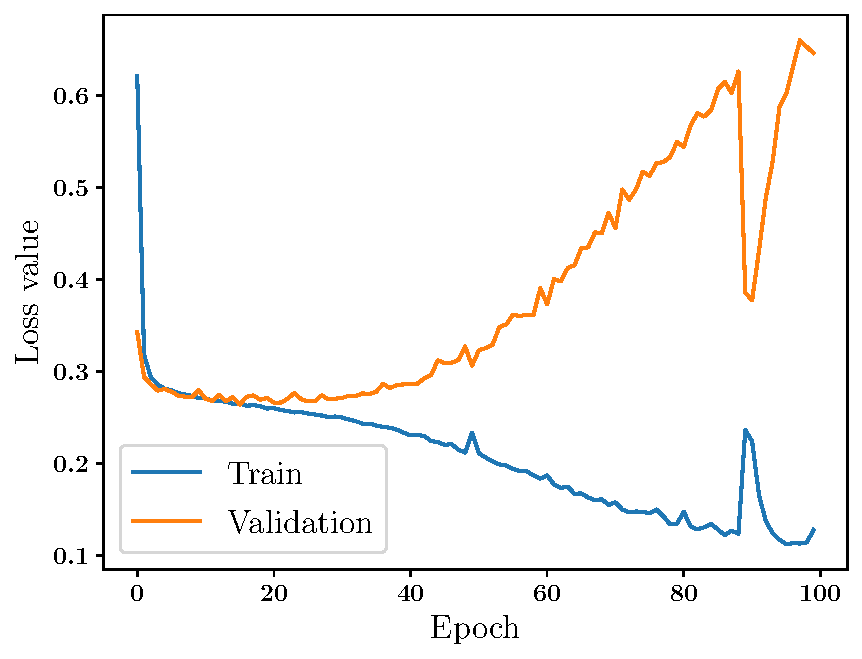
\includegraphics[width=\textwidth]{images/results/LB_test_10_20210613-180735__type_1branch_no_pool__st_scale_sub__lb_10__act_elu__nf_16__ks_10__nn_50__l2_1e-05__bs_200__ep_100__loss.pdf}
            \label{fig:lb_10_loss}
        }
    \end{minipage}%
    \hfill%
    \begin{minipage}[c]{0.49\textwidth}
        \vspace{0pt}
        \centering
        \subfloat[Accuracy with lookback $L=10$]{
        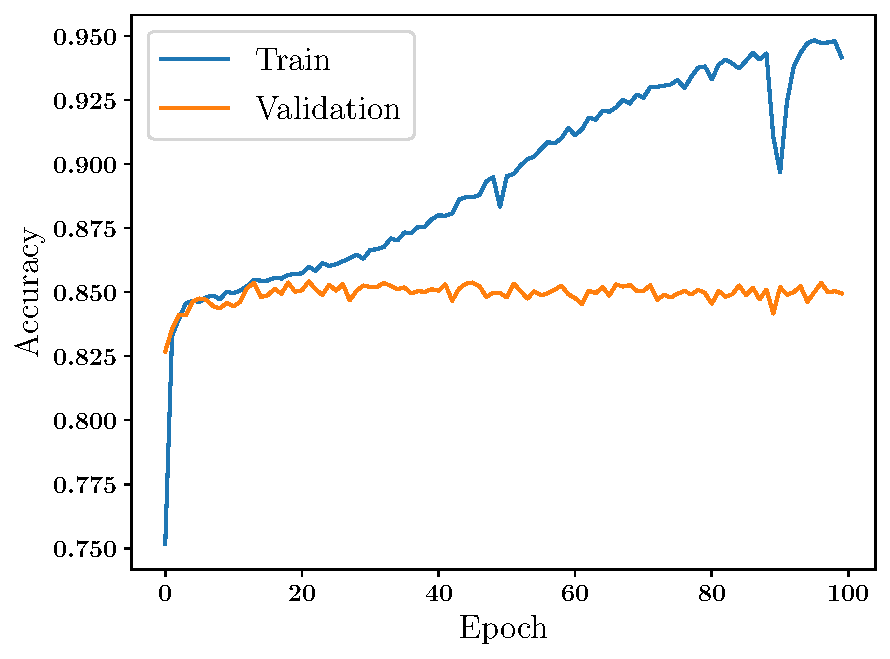
\includegraphics[width=\textwidth]{images/results/LB_test_10_20210613-180735__type_1branch_no_pool__st_scale_sub__lb_10__act_elu__nf_16__ks_10__nn_50__l2_1e-05__bs_200__ep_100___accuracy.pdf}
            \label{fig:lb_10_acc}
        }
    \end{minipage}
        \begin{minipage}[c]{0.49\textwidth}
        \vspace{0pt}
        \centering
        \subfloat[Loss function with lookback $L=20$]{
        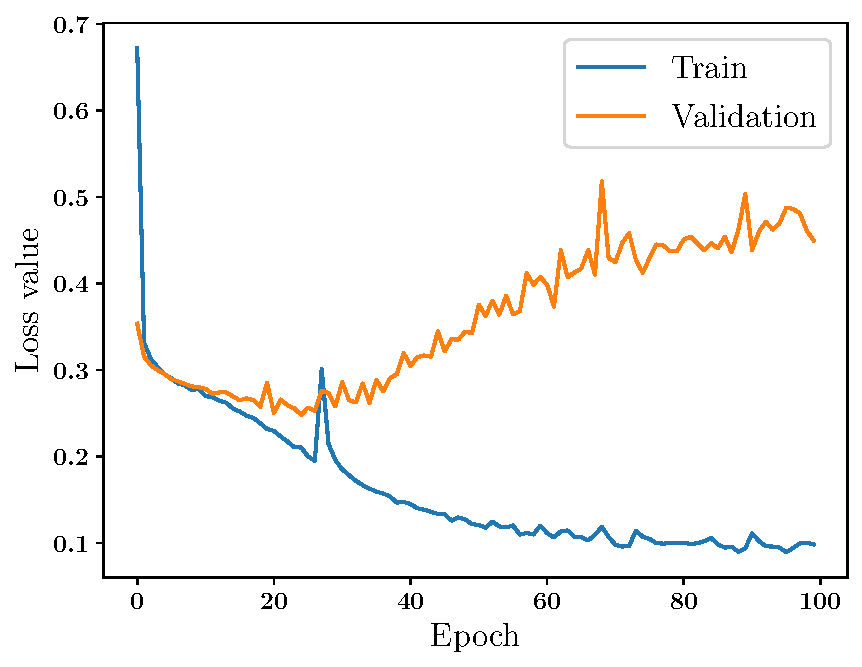
\includegraphics[width=\textwidth]{images/results/LB_test_20_20210613-180946__type_1branch_no_pool__st_scale_sub__lb_20__act_elu__nf_16__ks_10__nn_50__l2_1e-05__bs_200__ep_100__loss.pdf}
            \label{fig:lb_20_loss}
        }
    \end{minipage}%
    \hfill%
    \begin{minipage}[c]{0.49\textwidth}
        \vspace{0pt}
        \centering
        \subfloat[Accuracy with lookback $L=20$]{
        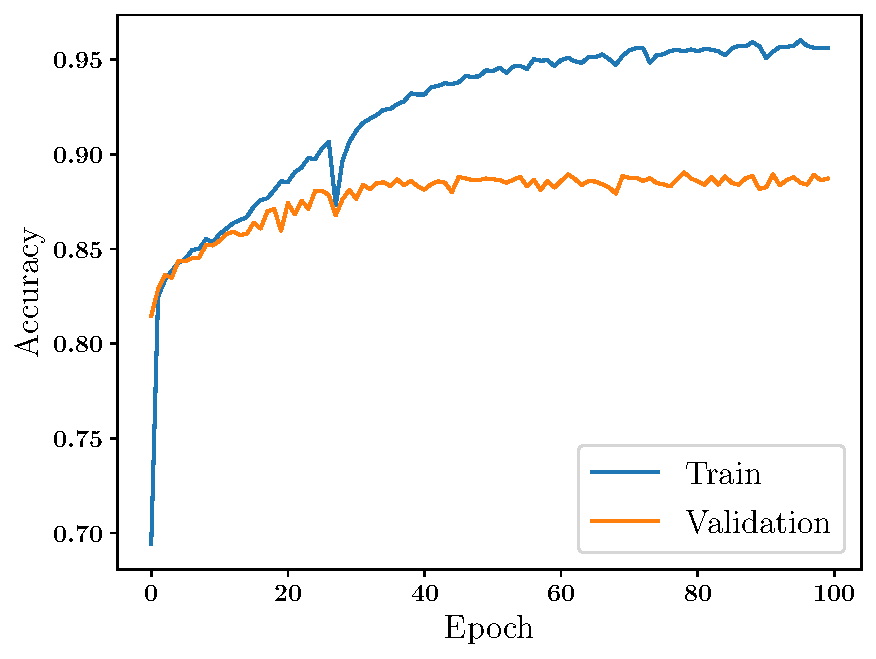
\includegraphics[width=\textwidth]{images/results/LB_test_20_20210613-180946__type_1branch_no_pool__st_scale_sub__lb_20__act_elu__nf_16__ks_10__nn_50__l2_1e-05__bs_200__ep_100___accuracy.pdf}
            \label{fig:lb_20_acc}
        }
    \end{minipage}    \begin{minipage}[c]{0.49\textwidth}
        \vspace{0pt}
        \centering
        \subfloat[Loss function with lookback $L=30$]{
        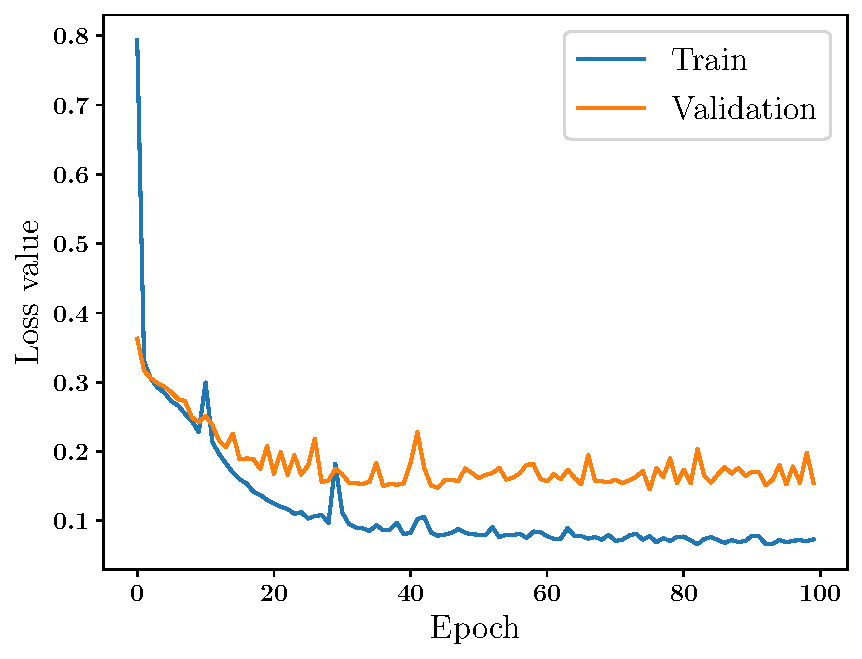
\includegraphics[width=\textwidth]{images/results/LB_test_30_20210613-181249__type_1branch_no_pool__st_scale_sub__lb_30__act_elu__nf_16__ks_10__nn_50__l2_1e-05__bs_200__ep_100__loss.pdf}
            \label{fig:lb_30_loss}
        }
    \end{minipage}%
    \hfill%
    \begin{minipage}[c]{0.49\textwidth}
        \vspace{0pt}
        \centering
        \subfloat[Accuracy with lookback $L=30$]{
        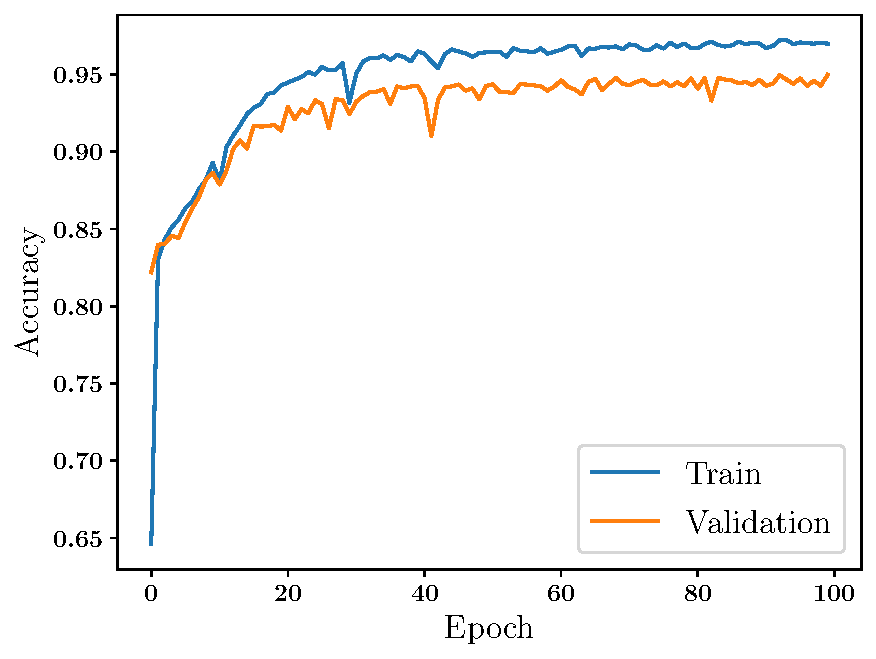
\includegraphics[width=\textwidth]{images/results/LB_test_30_20210613-181249__type_1branch_no_pool__st_scale_sub__lb_30__act_elu__nf_16__ks_10__nn_50__l2_1e-05__bs_200__ep_100___accuracy.pdf}
            \label{fig:lb_30_acc}
        }
    \end{minipage}


    \caption{lookback analysis}
    \label{fig:res_lb_val}
\end{figure}





\section{Model training and final performance}\label{res_test}

In this section we present the architecture and final performances of the proposed classifiers, after the training procedure, for both datasets. The performances have been evaluated using the test sets and the possible presence of over or under fitting behaviour is monitored, as shown previously, using the validation set. 

As previously said, the different size of the two dataset imposed the choice of implementing the 1B\_NP architecture, for the classification of the IoT dataset devices while, for the 4SICS dataset device classification, the 1B\_AP architecture was implemented. 
In \tabref{tab:final_models} we recall the main features of the two architectures, alongside with the chosen value of the hyperparameters introduced in \chapref{chap5}.

The behaviour of these models during the training, alongside with the final classification accuracy reached, is discussed in \secref{4sics_final_res} and \secref{iot_final_res} respectively for the 4SICS and IoT dataset.


%As previously said, for the 4SICS dataset, the 1B\_AP architecture was used while, for the %IoT dataset, the 1B\_NP one was implemented. Before showing the final results, in the %following list, we recall the main features and reported the chosen hyperparameters of these %classifier models:
%\begin{itemize}
%    \item Each convolutional layer contains 16 filters of size 10
%    \item Zero padding technique implementation in the 1B\_NP architecture
%    \item Pooling layers, if present, have pool size 2
%    \item ELU activation function and L2 regularization are implemented in each layer
%    \item Dropout rate of 30\% 
%    \item The first layer after the concatenation features 50 neurons, following layers have %each half neurons of the previous one
%    \item Adam optimizer and Categorical Crossentropy loss function
%\end{itemize}


%As previously said, for the 4SICS dataset, the 1B\_AP architecture was used while, for the %IoT dataset, the 1B\_NP one was implemented. Before showing the final results, we ropert n %\tabref{tab:final_models} the main features and the chosen hyperparameters of the used %classifier.

\begin{table}[h]
    \centering
    \begin{tabular}{lccm{5cm}}
    \Xhline{3\arrayrulewidth} 
       \multirow{2}{*}{\textbf{Parameter}}   &
       \multicolumn{2}{c}{\textbf{Dataset}} & \multirow{2}{*}{\textbf{Description}}\\
        & \textbf{4SICS dataset} & \textbf{IoT dataset} & 
       \\
    \Xhline{2\arrayrulewidth} 
        Architecture  & 1B\_AP & 1B\_NP & \footnotesize{Classifier architecture chosen from the ones shown in \chapref{chap5}}\\ \hline
        Filter number &\multicolumn{2}{c}{16} & \footnotesize{Number of filter contained in each convolutional layer} \\ \hline
        Filter dimension &\multicolumn{2}{c}{10} & \footnotesize{Dimension of the convolutional layer filters }\\ \hline
        Pool size  & 2 & $\boldsymbol{-}$ & \footnotesize{Pool dimension in pooling layers}\\ \hline
        Dropout Rate  &\multicolumn{2}{c}{30\%} &\footnotesize{ Probability of excluding a neuron in a dense layer}\\ \hline
        Number of neurons  & \multicolumn{2}{c}{50} & \footnotesize{Neurons in the first dense layer after concatenation }\\ \hline
        Optimizer    &\multicolumn{2}{c}{Adam} & \footnotesize{Optimization algorithm used to update the free parameters} \\ \hline
        Loss function  & \multicolumn{2}{c}{Categorical Crossentropy} & \footnotesize{Function to minimize during the training}\\ \hline
        Hidden layers activation & \multicolumn{2}{c}{ELU} & \footnotesize{Function applied to the output of each hidden layer} \\ \hline
        Final layers activation & \multicolumn{2}{c}{Softmax} & \footnotesize{Function applied to the final output of the classifier} \\ 
    \Xhline{3\arrayrulewidth}
    \end{tabular}
    \caption{Features and selected hyperparameters of the final classifier models. The results of the training and the final performance evaluation of these models are shown in \secref{4sics_final_res} and \secref{iot_final_res} respectively for the 4SICS and IoT dataset.}
    \label{tab:final_models}
\end{table}



\subsection{4SICS dataset}
\label{4sics_final_res}

The 1B\_AP model is trained using the samples, reported in \tabref{tab:4sicsdev}, obtained from the preprocess of the 4SICS dataset with a lookback value of $L=100$. The training is performed for 300 epochs using a batch size\footnote{The batch size indicates the number to use in the computation of the loss function during the training before updating the free parameters of the selected classifier.} of 200. 

In \figref{fig:4sics_results} the loss function and the model accuracy evolution, for both the training and validation set, is show. As we can see the model is able to reach high performances and does not show overfitting behaviour. 

After the training the final accuracy of the model is evaluated using the set, by comparing the predicted class of the devices with their true class. This comparison is done using a confusion matrix, shown in \figref{fig:4sics_results_cm}.\\
As we can see for all classes more than 90\% of the predicted labels are correct, with the Switch and Router class having 100\% correct predictions. From this matrix we also estimate a 96.2\% overall test accuracy.

\begin{figure}[!h]
    \centering
    \begin{minipage}[c]{0.49\linewidth}
        \vspace{0pt}
        \centering
        \subfloat[Loss function during training]{
        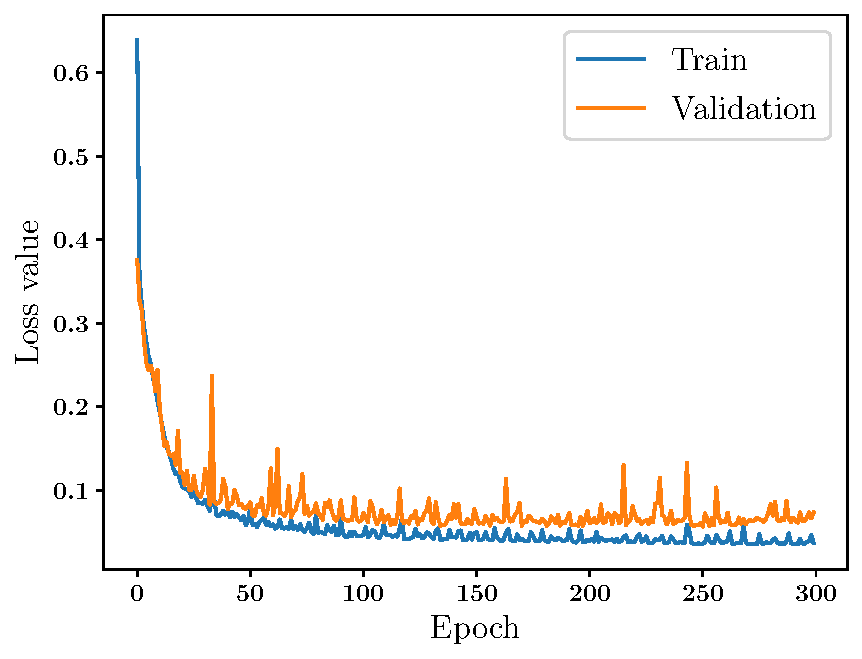
\includegraphics[width=\textwidth]{images/results/4SICS_clasf_20210613-174409__type_1branch__st_scale_sub__lb_100__act_elu__nf_16__ks_10__nn_50__l2_1e-05__bs_200__ep_300__loss.pdf}
            \label{fig:4sics_loss}
        }
    \end{minipage}%
    \hfill%
    \begin{minipage}[c]{0.49\linewidth}
        \vspace{0pt}
        \centering
        \subfloat[Accuracy during training]{  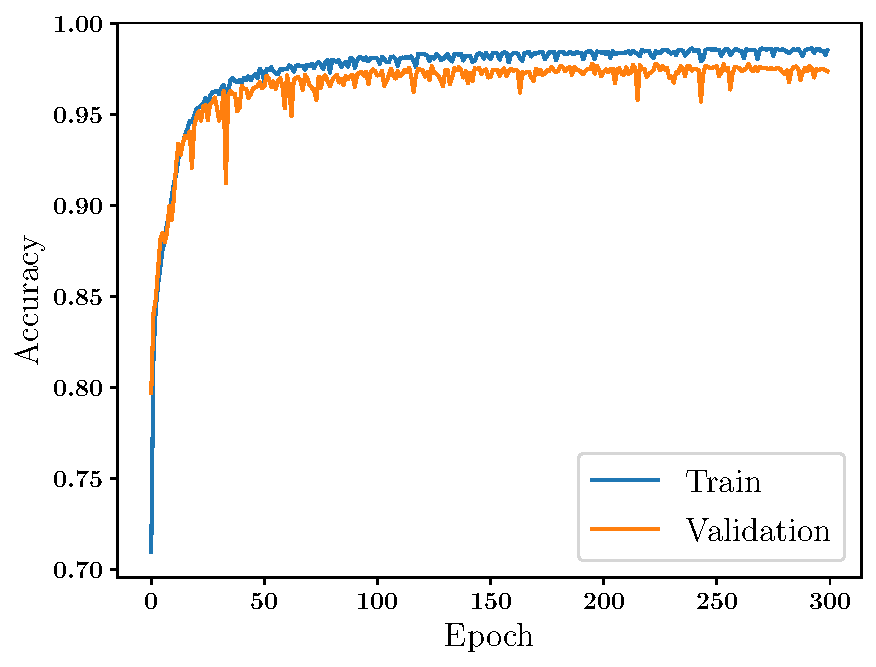
\includegraphics[width=\textwidth]{images/results/4SICS_clasf_20210613-174409__type_1branch__st_scale_sub__lb_100__act_elu__nf_16__ks_10__nn_50__l2_1e-05__bs_200__ep_300___accuracy.pdf}
        \label{fig:4sics_loss}
        }
    \end{minipage}%
    \caption{Model accuracy and loss function during training over both training and validation set. Results obtained during the training of the  1B\_AP architecture over the 4SICS dataset. }
    \label{fig:4sics_results}
\end{figure}


%
%\begin{figure}[h]
%    \centering
%        \includegraphics[width=0.6\textwidth]{images/results/4SICS_clasf_20210613-174409__typ%e_1branch__st_scale_sub__lb_100__act_elu__nf_16__ks_10__nn_50__l2_1e-05__bs_200__ep_3%00___cm.pdf}
%    \caption{Final 1B\_AP classifier predictions on 4SICS test set. Predictions are %visualized using a confusion matrix.  The colormap represents the fraction of samples %belonging to a certain prediction class.}
%    \label{fig:4sics_results_cm}
%\end{figure}


\begin{figure}[!h]
\begin{minipage}{0.6\linewidth}
    \centering
        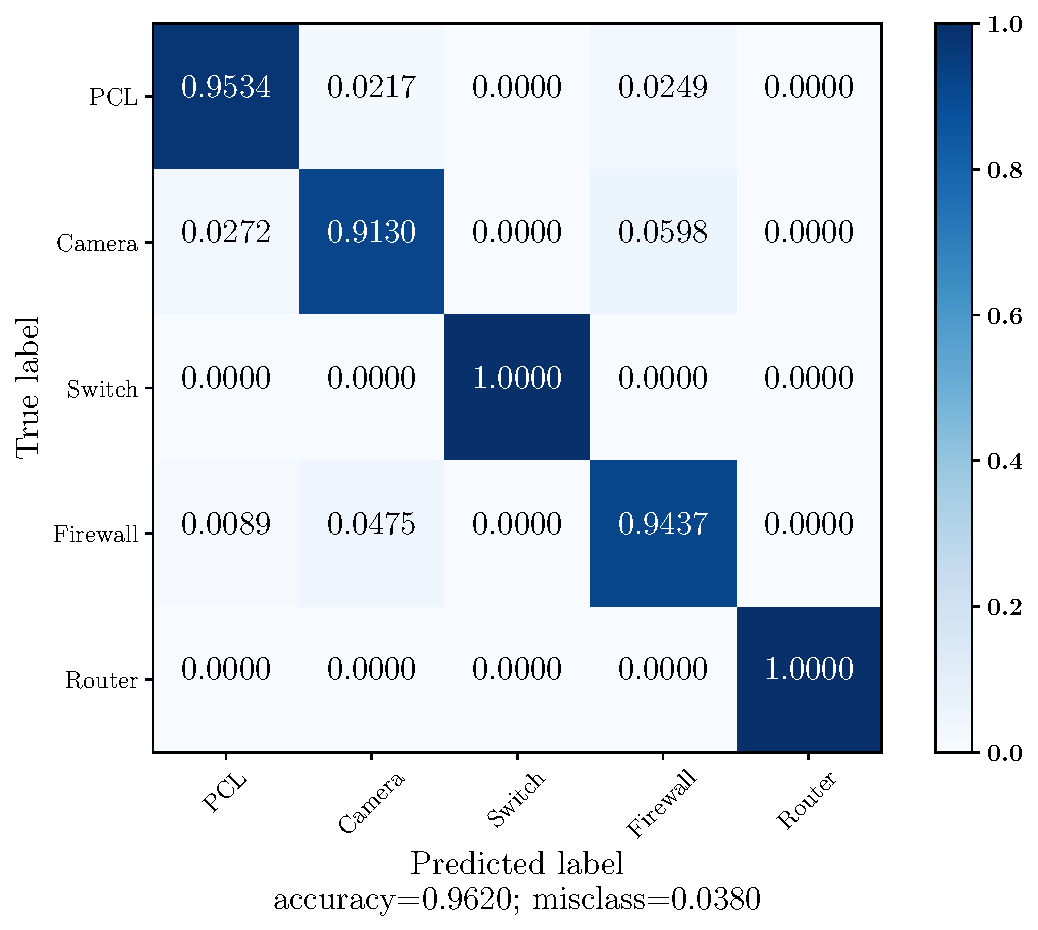
\includegraphics[width=\textwidth]{images/results/4SICS_clasf_20210613-174409__type_1branch__st_scale_sub__lb_100__act_elu__nf_16__ks_10__nn_50__l2_1e-05__bs_200__ep_300___cm.pdf}
\end{minipage}
\hfill
\begin{minipage}{0.29\linewidth}
\caption{Final 1B\_AP classifier predictions on 4SICS test set. Predictions are visualized using a confusion matrix.  The colormap represents the fraction of samples belonging to a certain prediction class.}
     \label{fig:4sics_results_cm}
\end{minipage}
\end{figure}



\subsection{IoT dataset}
\label{iot_final_res}


The 1B\_NP model is trained using the samples, reported in \tabref{tab:iotdev}, obtained from the preprocess of the IoT dataset with a lookback value of $L=30$. 

The training is performed for 300 epochs using a batch size of 100. 
In \figref{fig:iot_results} the loss function and the model accuracy evolution, for both the training and validation set, is show. Like for the previous case, also this model is able to reach high performances and does not show overfitting behaviour. 
As for the previous model we evaluate the final model accuracy using a confusion matrix, shown in \figref{fig:iot_results_cm}. In this case we observe a test accuracy higher than 95\%, for all the device classes, with an estimated overall test accuracy of 98.6\%
This result does also validate the chosen lookback value $L$ and architecture.

%As stated previously due to the small length of the timeseries the chosen architecture for %the device classification over the IoT Sentinel dataset in the 1B\_NP model, namely an %architecture with one convolutional "branch" without pooling layers. The selected device %classes, shown in \tabref{tab:iotdev}, have been preprocessed using a lookback $L=30$. The %training was performed for 300 epochs using a batch size of 100. 

%In \figref{fig:iot_results} the evolution of the loss function and of the model accuracy over %the training and validation set are shown. As for the previous dataset the model is able to %reach high performances and does not show overfitting behaviour, validating the choice of %architecture and lookback value. 
%

\begin{figure}[h]
    \centering
    \begin{minipage}[c]{0.49\linewidth}
        \vspace{0pt}
        \centering
        \subfloat[Loss function during training]{
        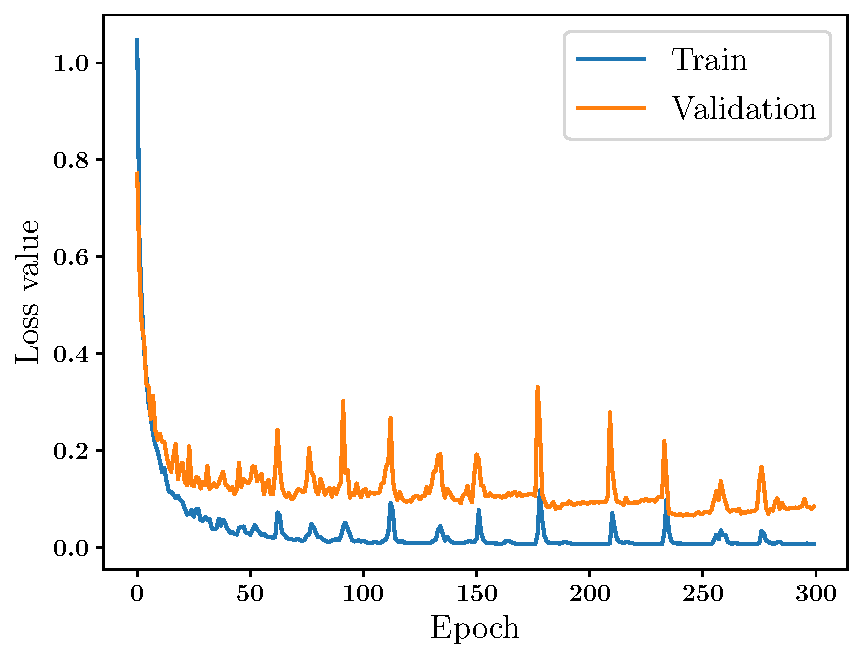
\includegraphics[width=\textwidth]{images/results/IoT_clasf_20210613-175027__type_1branch_no_pool__st_scale_sub__lb_30__act_elu__nf_16__ks_10__nn_50__l2_1e-05__bs_200__ep_300__loss.pdf}
            \label{fig:iot_loss}
        }
    \end{minipage}%
    \hfill%
    \begin{minipage}[c]{0.49\linewidth}
        \vspace{0pt}
        \centering
        \subfloat[Accuracy during training]{  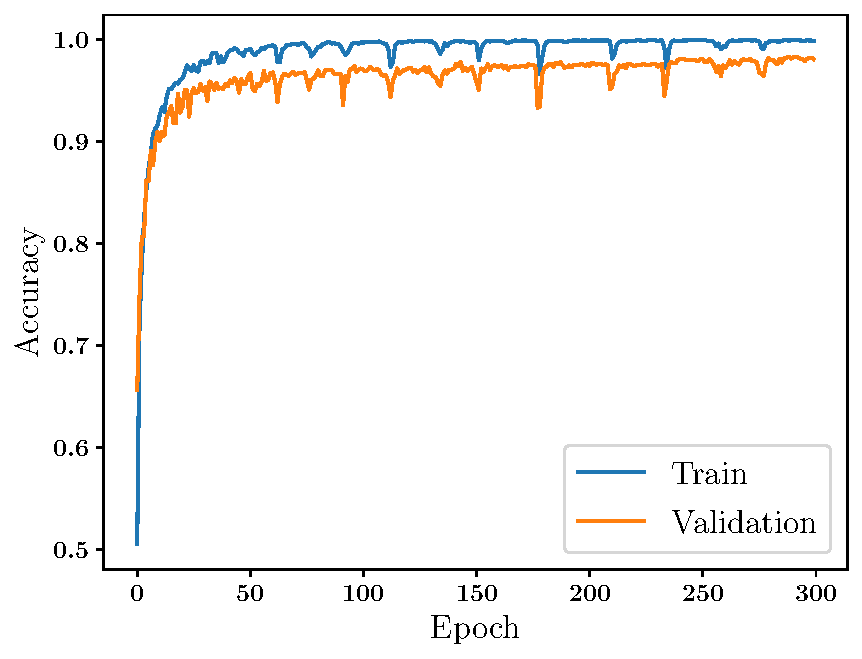
\includegraphics[width=\textwidth]{images/results/IoT_clasf_20210613-175027__type_1branch_no_pool__st_scale_sub__lb_30__act_elu__nf_16__ks_10__nn_50__l2_1e-05__bs_200__ep_300___accuracy.pdf}
        \label{fig:iot_loss}
        }
    \end{minipage}%
 \caption{Model accuracy and loss function during training over both training and validation set. Results obtained during the training of the  1B\_NP architecture over the IoT dataset. }       \label{fig:iot_results}
\end{figure}


%As for the previous model we evaluate the model performances using a confusion matrix, shown %in \figref{fig:4sics_results_cm}. For this dataset the classifier is able to reach a test %accuracy higher than 95\% for all the classes with an overall accurcay of 98.6\%

\begin{figure}[h]
\begin{minipage}{0.6\linewidth}
    \centering
        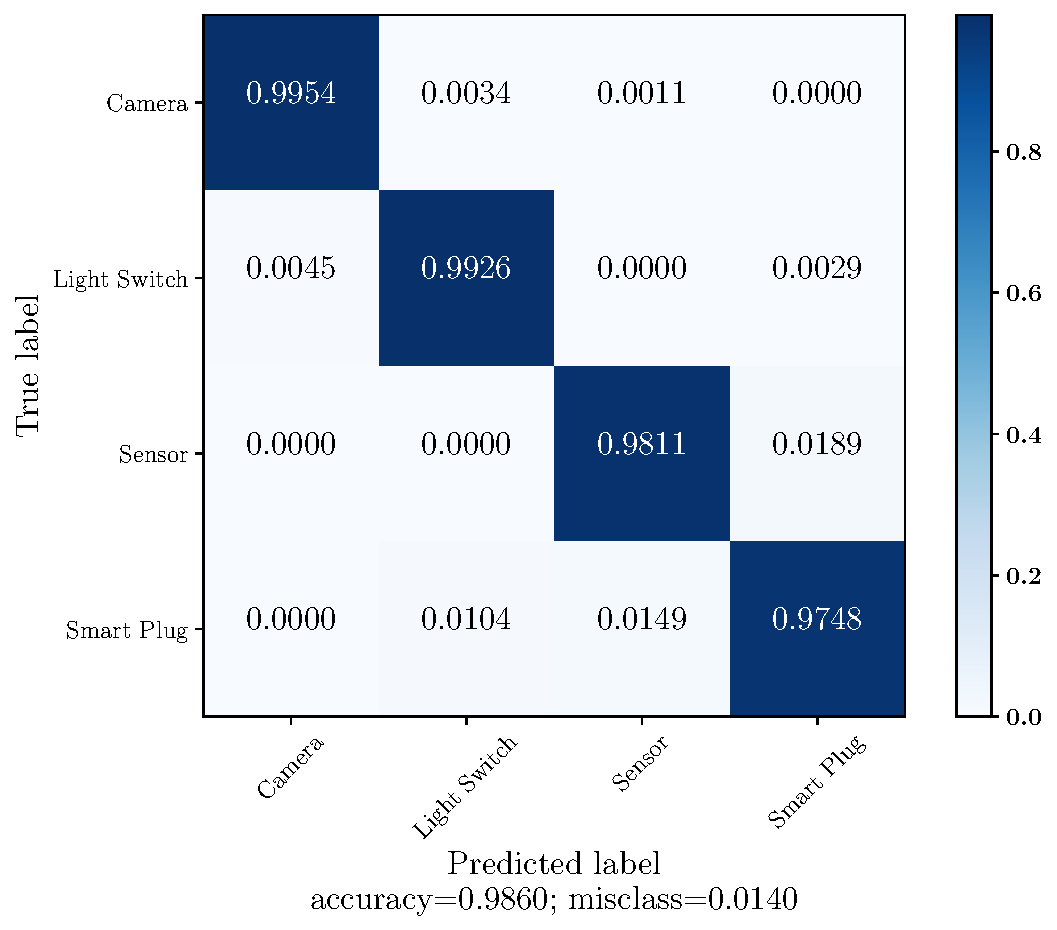
\includegraphics[width=\textwidth]{images/results/IoT_clasf_20210613-175027__type_1branch_no_pool__st_scale_sub__lb_30__act_elu__nf_16__ks_10__nn_50__l2_1e-05__bs_200__ep_300___cm.pdf}
\end{minipage}
\hfill
\begin{minipage}{0.29\linewidth}
  \caption{Final 1B\_NP classifier predictions on IoT Sentinel test set. Predictions are visualized using a confusion matrix.  The color map represents the fraction of samples belonging to a certain prediction class.} 
  \label{fig:iot_results_cm}
\end{minipage}
\end{figure}


\section{"Unseen" device classification}\label{res_unseen}

In the previous section we show that the proposed models are able, with great accuracy, of correctly of classifying a device. We now want to use the trained model in order to classify an "unseen" device.
More precisely our goal is to see if the classifier is able to recognize similarities between the device he was trained on and completely new devices. This test has is particularly interesting, due to how it translates in a real world application. In the real world in fact we can create more powerful classifiers, using deeper architecture or creating very big datasets with hundreds if not thousands of devices inside. The OT and IoT worlds however are continuously evolving and new devices are developed each year. The ability of the classifier of identifying a completely new device is then fundamental.

For each dataset we select two devices that were not included in the datasets described in \tabref{tab:4sicsdev} and \tabref{tab:iotdev}, but that belong to the device classes reported in them. We then processed their time series using exactly the same procedure and parameters as the one used to create the two training dataset. 
Once the new time series, with the respective communication protocol vector, are created, we use the trained classifiers to predict their device class. The final class prediction of the class of a device then corresponds to the class with the highest number of predicted time series. Thes result are shown as histograms in \figref{fig:4sics_unseen} and \figref{fig:iot_unseen} respectively for the 4SICS and IoT dataset. 



\begin{figure}[h]
    \centering
    \begin{minipage}[c]{0.49\linewidth}
        \vspace{0pt}
        \centering
        \subfloat[Class prediction of an "unseen" PLC]{
        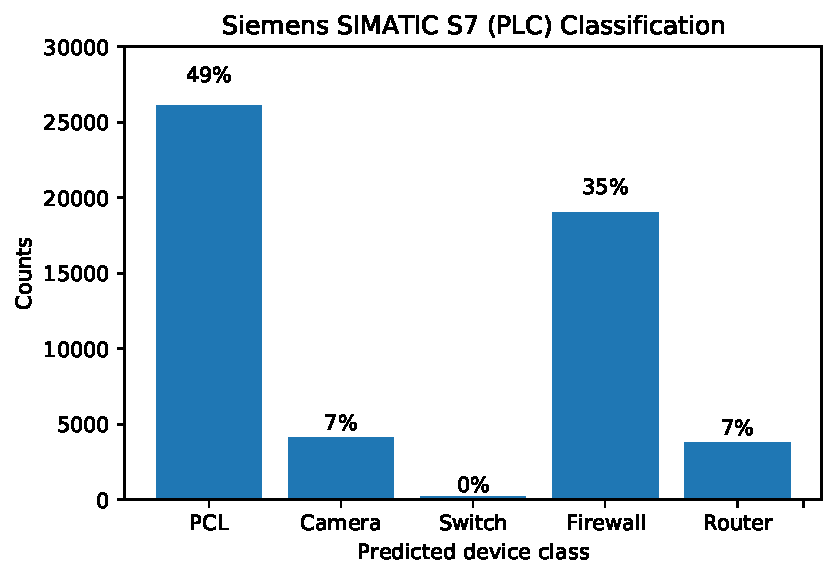
\includegraphics[width=\textwidth]{images/results/4sics_clasf_plc1_recognition.pdf}
            \label{fig:4sics_unseen_plc}
        }
    \end{minipage}%
    \hfill%
    \begin{minipage}[c]{0.49\linewidth}
        \vspace{0pt}
        \centering
        \subfloat[Class prediction of an "unseen" Router]
        {  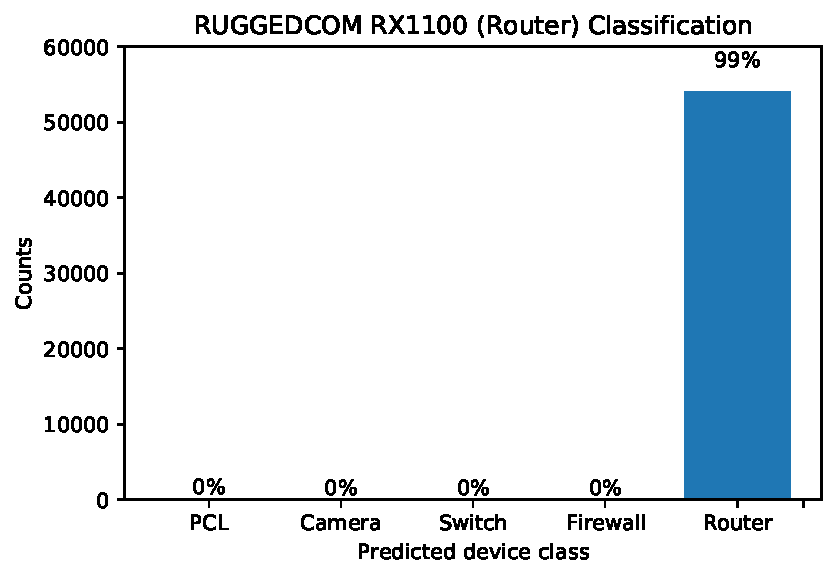
\includegraphics[width=\textwidth]{images/results/4sics_clasf_router_recognition.pdf}
            \label{fig:4sics_unseen_router}
        }
    \end{minipage}%
    \caption{Classification of "unseen" device using the trained 4SICS classifiers. Histogram shows the counts of time series assigned to each device class by the classifier. Selected devices belong to the PLC class, shown in \figref{fig:4sics_unseen_plc}, and Router class, shown in \figref{fig:4sics_unseen_router}; both devices are not included in the dataset shown in \tabref{tab:4sicsdev}.}
            \label{fig:4sics_unseen}
\end{figure}


\begin{figure}[!h]
    \centering
    \begin{minipage}[c]{0.49\linewidth}
        \vspace{0pt}
        \centering
        \subfloat[Class prediction of an "unseen" Camera]{
        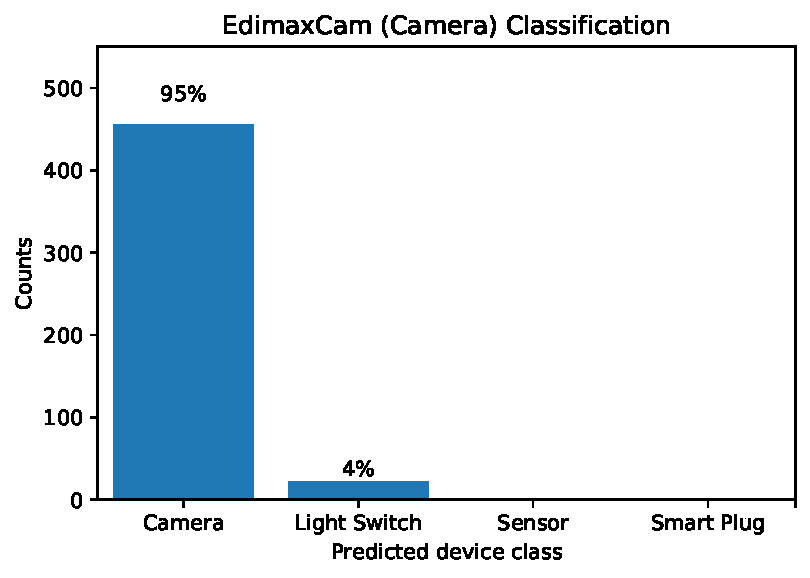
\includegraphics[width=\textwidth]{images/results/iot_clasf_cam_recognition.pdf}
            \label{fig:iot_unseen_camera}
        }
    \end{minipage}%
    \hfill%
    \begin{minipage}[c]{0.49\linewidth}
        \vspace{0pt}
        \centering
        \subfloat[Class prediction of an "unseen" Light Switch]
        {  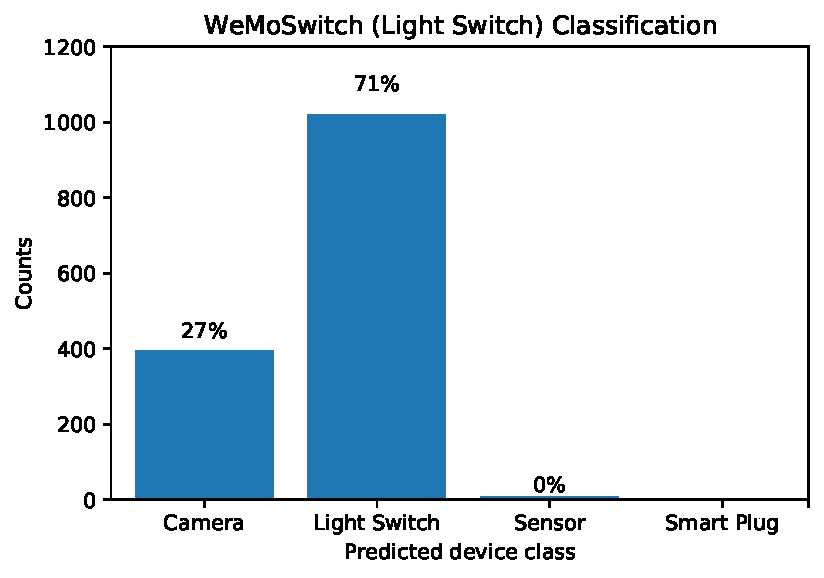
\includegraphics[width=\textwidth]{images/results/iot_clasf_switch_recognition.pdf}
            \label{fig:iot_unseen_light}
        }
    \end{minipage}%
 \caption{Classification of "unseen" device using the trained IoT Sentinel classifiers. Histogram shows the counts of time series assigned to each device class by the classifier. Selected devices belong to the Camera class, shown in \figref{fig:iot_unseen_camera}, and Light Switch class, shown in \figref{fig:iot_unseen_light}; both devices are not included in the dataset shown in \tabref{tab:iotdev}}
 \label{fig:iot_unseen}
\end{figure}

As we can see in all four cases the trained classifiers are able to correctly classify the "unseen" device. It is however important to notice that not all the predictions are done with the same accuracy. More specifically, we can see that, for the devices belonging to the Router and Camera class, more than 95\% time series have been correctly classified. The devices belonging to the PLC and Light Switch class on the other hand, despite being correctly classified, present a non negligible fraction of missclassified time series.

This can be expected since we are considering devices that were not part of the training dataset and the ability alone of the classifier of correctly identifying them is already a great achievement. A more precise classification can be achieved using larger training dataset with more included devices.


\section{Discussion}

In the previous sections we evaluated the performances of the proposed architectures over the two datasets. The results show that the classifiers are able to solve the identification task with great test accuracy. Looking at the loss function and accuracy plot we see a regular behaviour, allowing us to exclude the presence of over or under fitting. This fact, alongside with the overall test accuracy obtained, validates the choice made for the architecture and lookback value in both situations as well as the overall proposed approach.

Looking at the presented confusion matrices we estimated the overall test accuracy, obtaining very high values in both cases. This translates, in a real world application, in the ability, of a trained classifier, of correctly recognizing a device that was included in its training dataset with great precision.

The use of trained classifier to identify devices not included in the training dataset show that the proposed architectures are able to recognize similarities in the device behaviour and, consequently, of correctly classifying them. This result is really important since it demonstrates the capability, of a trained classifier, to easily adapt to new devices and technologies. In a real world application this translates in the possibility of truly implementing this type of classifier as a device identifier, without the necessity of executing a new training procedure whenever a newly developed device is connected to the supervised network.
\chapter{Conclusions}

\lipsum[1-8]



%
\appendix
\chapter{Alternative Classifier Structures} 
\label{app:2bmodel}
\textbf{\large FOTO 2 branch convo}

\chapter{Appendix B}
\backmatter

\begin{thebibliography}{99}

\renewcommand{\baselinestretch}{1} 


\bibitem{perceptron}
\textit{The perceptron: a probabilistic model for information storage and organization in the brain}
\\\url{http://citeseerx.ist.psu.edu/viewdoc/summary?doi=10.1.1.335.3398}

\bibitem{nielsen}
\textit{Neural Networks and Deep Learning}
\\\url{http://neuralnetworksanddeeplearning.com}

\bibitem{relu}
\textit{Deep Learning using Rectified Linear Units (ReLU)}
\\\url{https://arxiv.org/pdf/1803.08375.pdf}

\bibitem{elu}
\textit{Fast and Accurate Deep Network Learning by Exponential Linear Units (ELUs)}
\\\url{https://arxiv.org/abs/1511.07289}

\bibitem{gelu}
\textit{Gaussian Error Linear Units (GELUS)}
\\\url{https://arxiv.org/pdf/1606.08415.pdf}

\bibitem{lossfunc}
\textit{On Loss Functions for Deep Neural Networks
in Classification}
\\\url{https://arxiv.org/pdf/1702.05659.pdf}

\bibitem{kullbackeff}
\textit{Optimism in Reinforcement Learning and Kullback-Leibler Divergence
}
\\\url{https://arxiv.org/abs/1004.5229}

\bibitem{kullbackeff2}
\textit{Why Deep Learning Methods Use KL Divergence
Instead of Least Squares: A Possible Pedagogical
Explanation}
\\\url{https://scholarworks.utep.edu/cgi/viewcontent.cgi?article=2188&context=cs_techrep}



\bibitem{overfitting}
\textit{An Overview of Overfitting and its Solutions}
\\\url{https://arxiv.org/pdf/1609.04747.pdf}


\bibitem{backprop}
\textit{An Overview of Overfitting and its Solutions}
\\\url{Learning representations by back-propagation errors}

\bibitem{var_grad}
\textit{An overview of gradient descent optimization
algorithms}
\\\url{Learning representations by back-propagation errors}

\bibitem{adam}
\textit{Adam: A Method for Stochastic Optimization}
\\\url{https://arxiv.org/abs/1412.6980}

\bibitem{bert}
\textit{BERT: Pre-training of Deep Bidirectional Transformers for
Language Understanding}
\\\url{https://arxiv.org/pdf/1810.04805.pdf}

\bibitem{gpt}
\textit{Language Models are Unsupervised Multitask Learners}
\\\url{https://cdn.openai.com/better-language-models/language_models_are_unsupervised_multitask_learners.pdf}



\bibitem{l1reg}
\textit{L1 regularization is better than L2 for learning and predicting chaotic systems
}
\\\url{https://arxiv.org/pdf/cs/0410015.pdf}

\bibitem{l2reg}
\textit{$L_2$ Regularization for Learning Kernels}
\\\url{https://arxiv.org/pdf/1205.2653.pdf}

\bibitem{srivastava}
\textit{Dropout: A Simple Way to Prevent Neural Networks from Overfitting}
\\\url{http://jmlr.org/papers/volume15/srivastava14a/srivastava14a.pdf}


\bibitem{webfingerprint1}
\textit{The Web never forgets: Persistent tracking mechanisms in the wild}
\\\texttt{Proc. ACM SIGSAC Conf. Comput. Commun. Secur. Secur., pp. 674-689}

\bibitem{webfingerprint2}
\textit{FPDetective: Dusting the web for fingerprinters}
\\\texttt{Proc. ACM SIGSAC Conf. Comput. Commun. Secur., pp. 1129-1140}

\bibitem{radiofingerprint}
\textit{Wireless device identification with radiometric signatures}
\\\texttt{Proc. ACM SIGSAC Conf. Comput. Commun. Secur., pp. 1129-1140}

\bibitem{idos1}
\textit{Passive OS fingerprinting by DNS traffic analysiss}
\\\url{https://ieeexplore.ieee.org/document/6531762}

\bibitem{idos2}
\textit{Study on OS fingerprinting and nat/tethering based on DNS log analysis}
\\\url{https://irtf.org/raim-2015-papers/raim-2015-paper21.pdf}


\bibitem{iot_2020}
\textit{How the ’Internet of Things’ will impact consumers,
businesses, and governments in 2016 and beyond.}
\\\url{http://www.businessinsider.de/how-the-internet-of-things-market-will-grow-2014-10}

\bibitem{attk1}
\textit{AVTECH DVR multiple vulnerabilities.}
\\\url{https://www.coresecurity.com/core-labs/advisories/avtech-dvr-multiple-vulnerabilities}

\bibitem{attk2}
\textit{Hacking a Wi-Fi coffee machine – part 1.}
\\\url{https://www.pentestpartners.com/security-blog/hacking-a-wi-fi-coffee-machine-part-1/}

\bibitem{flaw}
\textit{400,000 publicly available IoT devices vulnerable to single
flaw.}
\\\url{https://blog.senr.io/blog/400000-publicly-available-iot-devices-vulnerable-to-single-flaw}

\bibitem{clasf}
\textit{Supervised machine learning: a review of classification techniques.}
\\\url{https://dl.acm.org/doi/10.5555/1566770.1566773}

\bibitem{imbclasf}
\textit{Survey on deep learning with class imbalance.}
\\\url{https://journalofbigdata.springeropen.com/articles/10.1186/s40537-019-0192-5}


\bibitem{4sics_site}
\textit{Capture files from 4SICS Geek Lounge}
\\\url{https://www.netresec.com/?page=PCAP4SICS}

\bibitem{iot_site}
\textit{IoT devices captures. Aalto University}
\\\url{https://research.aalto.fi/en/datasets/iot-devices-captures}

\bibitem{iot_paper}
\textit{IOT SENTINEL: Automated Device-Type
Identification for Security Enforcement in IoT}
\\\url{https://arxiv.org/pdf/1611.04880.pdf}

\bibitem{python}
\textsc{Python 3} Documentation
\\\url{https://docs.python.org/3/}

\bibitem{numpy}
\textsc{Numpy} Documentation
\\\url{https://numpy.org/doc/}

\bibitem{pandas}
\textsc{Pandas} Documentation
\\\url{https://pandas.pydata.org/docs/}

\bibitem{wireshark}
\textsc{Wireshark} Documentation
\\\url{https://www.wireshark.org/download/docs/user-guide.pdf}


\bibitem{gce}
\textit{Nozomi Networks Guardian Community Edition}
\\\url{https://community.nozominetworks.com/}

\bibitem{nozomi}
\textsc{Nozomi Networks} website
\\\url{https://www.nozominetworks.com/}

 
\bibitem{tf} 
\textsc{TensorFlow} Documentation 
\\\url{https://www.tensorflow.org/guide}

\bibitem{keras} 
\textsc{Keras} Documentation 
\\\url{https://keras.io/}







\end{thebibliography}

%\printbibliography

\end{document}